\chapter{Unitarity and Sum-Rule Bounds in the Standard Model Effective Field Theory\label{ch:SMEFT_bounds}}

\begin{flushright}
\small

{\color{chapterpaperrule}\rule{\textwidth}{0.5pt}}

\textit{This chapter is based on Ref.~\cite{Bresciani:2026acy}:}\\[0.5em]
L.~C.~Bresciani, P.~Paradisi and A.~Sainaghi,\\[0pt]
``Unitarity bounds and sum rules in the SMEFT,''\\[0pt]
[\href{https://doi.org/10.48550/arXiv.2603.03423}{arXiv:2603.03423} [hep-ph]].

{\color{chapterpaperrule}\rule{\textwidth}{0.5pt}}
\end{flushright}

\section{Introduction}

The discovery of a scalar particle consistent with the SM Higgs boson at the LHC has firmly
established the validity of the SM. Since no experimental data at present significantly contradict
the SM predictions, it is customary to assume the emergence of new physics at energies much above the
electroweak scale. In this context, EFTs provide a systematic framework to parameterize possible
deviations from the SM by introducing higher-dimensional operators constructed from the SM fields and
respecting its symmetries, namely the
SMEFT~\cite{Buchmuller:1985jz,Grzadkowski:2010es,Brivio:2017vri,Isidori:2023pyp,Aebischer:2025qhh}.

As discussed in Chapter~\ref{ch:generalizedUB}, a key theoretical consistency requirement for any theory
is perturbative unitarity, derived from the fundamental properties of the scattering
$S$-matrix~\cite{Jacob:1959at}. The resulting bounds are inherently perturbative, being derived at
tree level, and therefore do not represent sharp exclusions. Their saturation signals the breakdown
of the low-energy description, indicating the energy scale at which new degrees of freedom or a
strongly coupled regime must appear.

Partial-wave unitarity bounds within the SMEFT have already been partially explored in the
literature. In particular, Refs.~\cite{Corbett:2014ora,Corbett:2017qgl,Cao:2023qks} considered
dimension-six bosonic operators and two-fermion-two-boson operators, but restricted the analysis to
operators without gluon fields. In these works, four-fermion operators were not considered. Earlier
studies addressed unitarity in specific four-fermion interactions~\cite{Anders:1993dk}, but a
systematic SMEFT treatment was still lacking. Moreover, dimension-six operators $\psi^2\varphi^3$
modifying the Yukawa interactions were neglected, and no unitarity bounds were derived for the Higgs
operator $(\varphi^\dagger \varphi)^3$.
In this chapter we fill these gaps by providing the first complete coupled-channel implementation of
perturbative unitarity for the baryon-number-conserving dimension-six SMEFT. To this end, we compute
all relevant scattering amplitudes including every allowed helicity, gauge, and flavor configuration,
consistently retaining the correlations among Wilson coefficients entering the same partial-wave
amplitudes. We then marginalize over each Wilson coefficient. This is especially relevant in flavor
scenarios with dominant couplings to third-generation fermions, as naturally realized in models
addressing the flavor puzzle at the TeV scale, which have attracted considerable interest in the
recent
literature~\cite{Bordone:2017bld,Greljo:2018tuh,Allwicher:2020esa,Fuentes-Martin:2020bnh,%
Fuentes-Martin:2022xnb,Barbieri:2023qpf,Barbieri:2024zkh,Davighi:2023evx,Davighi:2023iks,%
Fuentes-Martin:2024fpx,Covone:2024elw,Lizana:2024jby,FernandezNavarro:2023rhv,%
FernandezNavarro:2024hnv,FernandezNavarro:2025zmb,Isidori:2025rci,Greljo:2025mwj}.

The analyticity of the $S$-matrix allows one to derive spin-dependent sum
rules~\cite{Low:2009di,Altmannshofer:2023bfk,Altmannshofer:2025lun,Gu:2020thj,Azatov:2021ygj,%
Remmen:2020uze,Remmen:2022orj}, providing additional theoretical constraints on effective
four-fermion interactions beyond the partial-wave unitarity bounds. Remarkably, the resulting pattern
of SMEFT inequalities can be used to infer characteristic features of the underlying new-physics
dynamics, indicating whether it is dominated by scalar or vector states. A further goal of this
chapter is therefore to explore the complementarity of unitarity and sum-rule constraints, as well as
their competitiveness with both current and projected experimental limits.

In the high-energy particle physics community, there is a growing consensus on performing
new-physics searches with minimal theoretical priors. The huge and otherwise unmanageable parameter
space must be supplemented by restrictive, yet general, first-principles criteria to make such
searches tractable. In this context, the results of this chapter provide a systematic consistency
framework that can be directly incorporated into present and future global SMEFT analyses.

The chapter is organized as follows. In Section~\ref{sec:SMEFT_unitaritybounds} we apply the method
of Chapter~\ref{ch:generalizedUB} to the dimension-six SMEFT and collect the marginalized bounds on
the complete set of Wilson coefficients in the single-flavor limit. In
Section~\ref{sec:SMEFT_sumrules} we derive the spinning sum rules for four-fermion operators in the
Warsaw basis, describing how they are turned into inequalities on the Wilson coefficients and under
which conditions they may fail. In Section~\ref{sec:SMEFT_multiflavor} we present the bounds on four-fermion operators under the MFV and $U(2)^5$ flavor
hypotheses. Section~\ref{sec:SMEFT_pheno} is dedicated to the phenomenological applications of our
results and to their interplay with current and projected experimental limits. Our conclusions are
presented in Section~\ref{sec:SMEFT_conclusions}. Finally, Appendix~\ref{app:SMEFT_conv} collects the
operator basis and our conventions, Appendix~\ref{app:SMEFT_UV} matches a representative set of
UV completions onto the semileptonic operators, Appendix~\ref{app:SMEFT_math} gathers the
mathematical tools used in the derivation of the bounds, and Appendix~\ref{app:SMEFT_flavorresults}
reports the complete set of bounds on the flavorful four-fermion operators.

\section{Unitarity Bounds\label{sec:SMEFT_unitaritybounds}}

To compute the unitarity bounds, we adopt the method developed in Chapter~\ref{ch:generalizedUB}, which allows one to project a generic scattering amplitude $\ket*{\mathcal{A}_{i\to f}}$ onto a kinematic basis $\ket*{\mathcal{B}^J_{i\to f}}$ with definite angular momentum $J$, as follows:
\begin{equation}
\ket*{\mathcal{A}_{i\to f}}=\sum_J a_{i\to f}^J \ket*{\mathcal{B}_{i\to f}^J}\,,
\end{equation}
where $a_{i\to f}^J$ denote the partial-wave coefficients and the elements of the kinematic basis are normalized as 
\begin{equation}
    \langle \mathcal B^J_{i\to f}|\mathcal B^{J'}_{i\to f}\rangle = \int \dd\Phi_i \dd\Phi_f \, \mathcal B^{J'}_{i\to f} \left(\mathcal B^J_{i\to f}\right)^* = (2J+1)\delta^{JJ'}\,,
\end{equation}
where $\dd\Phi_{i,f}$ refers to the phase-space measure associated with the initial and final states.
In terms of $a_{i\to f}^J$, the partial-wave unitarity bounds 
take the form
%
\begin{equation}\label{unitarity bound general}
\abs*{\Re a_{i\to i}^J}\leq 1\,,
\quad
0\leq \Im a_{i\to i}^J\leq 2\,,
\quad
\abs*{a_{i\to f}^J}\leq 1\,,
\end{equation}
with $i \neq f$.
Further details on the construction of the basis and on the derivation of these bounds have been given in Chapter~\ref{ch:generalizedUB}.

Using this framework, we systematically computed the partial-wave unitarity bounds 
for all dimension-six SMEFT Wilson coefficients in the Warsaw basis \cite{Grzadkowski:2010es}, reported in Appendix~\ref{app:SMEFT_conv} with the relevant conventions. 
The resulting bounds in the single-flavor limit are summarized in Table~\ref{tab:UniBounds}.

\begin{table}[h!t!b]
\renewcommand{\arraystretch}{1.5}
    \centering
    \resizebox{\textwidth}{!}{
    \begin{tabular}{c|c|c|c|c|c|c|c|c|c}
    \toprule
    \rowcolor{hdrcolor}
    \multicolumn{2}{c|}{{\boldmath$X^3$}} & \multicolumn{2}{c|}{{\boldmath$\varphi^6$} and {\boldmath$\varphi^4D^2$}} & \multicolumn{2}{c|}{{\boldmath$   \psi^2\varphi^3$}} & \multicolumn{2}{c|}{{\boldmath$(\overline{L}L)(\overline{L}L)$}} & \multicolumn{2}{c}{{\boldmath$(\overline{L}R)(\overline{R}L)$} and {\boldmath$(\overline{L}R)(\overline{L}R)$}}\\
    \hline
    $C_G$ & $4\pi/(9g_s)$ & $C_\varphi$ & $32\pi^3/3$ & $C_{e\varphi}$ & $32\pi^2/\sqrt{3}$ & $C_{\ell\ell}$ & $2\pi$ & $C_{\ell e dq}$ & $8\pi/\sqrt{3}$ \\
    
    $C_{\widetilde G}$ & $4\pi/(9g_s)$ & $C_{\varphi\Box}$ & $8\pi/3$ & $C_{u\varphi}$ & $32\pi^2/3$ & $C_{qq}^{(1)}$ & $6\pi/5$ & $C_{quqd}^{(1)}$ & $16\pi(1+\sqrt{2})/9$\\ 
        
    $C_W$ & $2\pi/(3g)$ &$C_{\varphi D}$ & $32\pi/3$ & $C_{d\varphi}$ & $32\pi^2/3$ & $C_{qq}^{(3)}$ & $4\pi/3$ & $C_{quqd}^{(8)}$ & $4\pi(2+7\sqrt{2})/3$\\
    
    $C_{\widetilde W}$ & $2\pi/(3g)$ & & & & & $C_{\ell q}^{(1)}$ & $2\pi\sqrt{3}$ & $C_{\ell equ}^{(1)}$ & $8\pi/\sqrt{3}$ \\

    &&&&&&  $C_{\ell q}^{(3)}$ & $2\pi$ & $C_{\ell e qu}^{(3)}$ & $(2+\sqrt{2})\pi/3$   \\
    
         \midrule
         \rowcolor{hdrcolor}
         \multicolumn{2}{c|}{{\boldmath$X^2\varphi^2$}} & \multicolumn{2}{c|}{{\boldmath$\psi^2 X \varphi$}} & \multicolumn{2}{c|}{{\boldmath$\psi^2\varphi^2D$}} & \multicolumn{2}{c|}{{\boldmath$(\overline{R}R)(\overline{R}R)$}} & \multicolumn{2}{c}{{\boldmath$(\overline{L}L)(\overline{R}R)$}}\\
         \hline
         $C_{\varphi G}$ & $\pi$ & $C_{eW}$ & $4\pi\sqrt{2/3}$ & $C_{\varphi \ell}^{(1)}$ & $8\pi$ & $C_{ee}$ & $2\pi$ & $C_{\ell e}$ & $4\pi$ \\
         
         $C_{\varphi \widetilde G}$ & $\pi$ & $C_{eB}$ & $4\pi$ & $C_{\varphi \ell}^{(3)}$ & $8\pi/3$ & $C_{uu}$ & $3\pi/2$ & $C_{\ell u}$ & $4\pi$\\
         
         $C_{\varphi W}$ & $2\pi\sqrt{2/3}$ & $C_{uG}$ & $2\pi\sqrt{3}$ & $C_{\varphi e}$ & $8\pi$ & $C_{dd}$ & $3\pi/2$ & $C_{\ell d}$ & $4\pi$\\
         
         $C_{\varphi \widetilde W}$ & $2\pi\sqrt{2/3}$ & $C_{uW}$ & $4\pi\sqrt{2/3}$ & $C_{\varphi q}^{(1)}$ & $2\pi\sqrt{6}$ & $C_{eu}$ & $4\pi$ & $C_{q e}$ & $4\pi$ \\
         
        $C_{\varphi B}$ & $2\pi\sqrt{2}$ & $C_{uB}$ & $4\pi$ & $C_{\varphi q}^{(3)}$ & $8\pi/3$ & $C_{ed}$ & $4\pi$ & $C_{q u}^{(1)}$ & $2\pi\sqrt{2}$\\
        
        $C_{\varphi \widetilde B}$ & $2\pi\sqrt{2}$ & $C_{dG}$ & $2\pi\sqrt{3}$ & $C_{\varphi u}$ & $4\pi \sqrt{3}$ & $C_{ud}^{(1)}$ & $4\pi$ & $C_{q u}^{(8)}$ & $3\pi(1+1/\sqrt{2})$\\
        
        $C_{\varphi W B}$ & $4\pi$ & $C_{dW}$ & $4\pi\sqrt{2/3}$ & $C_{\varphi d}$ & $4\pi\sqrt{3}$ & $C_{ud}^{(8)}$ & $8\pi$ & $C_{qd}^{(1)}$ & $2\pi\sqrt{2}$\\
        
        $C_{\varphi \widetilde W B}$ & $4\pi$ & $C_{dB}$ & $4\pi$ & $C_{\varphi ud}$ & $8\pi$ & & & $C_{q d}^{(8)}$ & $3\pi(1+1/\sqrt{2})$ \\
        \bottomrule
    \end{tabular}
    }
    \caption{Unitarity bounds on the modulus of the baryon-number-conserving dimension-six SMEFT Wilson coefficients in the Warsaw basis \cite{Grzadkowski:2010es} (see Table \ref{tab:WarsawBasis}), obtained by marginalizing over all other SMEFT coefficients. The factors $s/\Lambda^2$ are left implicit, i.e., the reported values constrain the combination $s|C|/\Lambda^2$. Fermionic operators correspond to the single-flavor limit.}
    \label{tab:UniBounds}
\end{table}

Several comments are in order. 
In contrast to the common practice in SMEFT analyses, where only one or a few operators are considered at a time, the unitarity bound associated with each Wilson coefficient is obtained by marginalizing over all other SMEFT coefficients. 
In practice, the marginalized bound on each coefficient is its largest value allowed by unitarity with all remaining coefficients free to vary. Since the partial-wave coefficients depend linearly on the Wilson coefficients,
Eq.~\eqref{unitarity bound general} carves out a convex region in coefficient space,
and each marginalized bound is the projection of this region onto the corresponding
axis. Moreover, since all scattering channels are considered, the region is bounded. Indeed, by the amplitude/operator correspondence, the number of independent amplitudes equals that of independent operators, so that the unitarity conditions constrain every possible direction in coefficient space. Thus, the numbers in Table~\ref{tab:UniBounds} should be interpreted as conservative one-dimensional projections of the full coupled-channel unitarity region, rather than as single-operator bounds.
This procedure is particularly relevant for coefficients that contribute to the same scattering amplitudes. This occurs for the following classes of operators:
\begin{itemize}
    \item $O_{\varphi \Box}$ and $O_{\varphi D}$;
    \item All pairs involving either a field-strength tensor $X$ or its dual $\widetilde X$;
    \item All pairs containing fermionic bilinears in the singlet or triplet (octet) representations of $SU(2)$ ($SU(3)$).
\end{itemize}
Representative examples are shown in Figures~\ref{fig:uni3} and \ref{fig:1-flavor unitary+sum rules}.

% \begin{figure}[htbp]
%     \centering
%     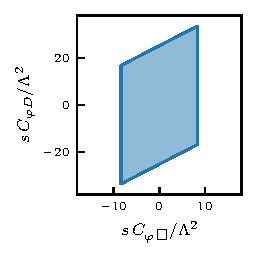
\includegraphics[scale=1.25]{images/C_H4D2.pdf}\quad
%     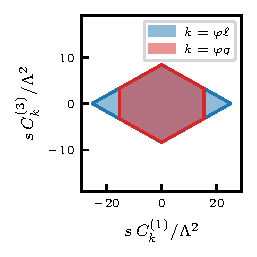
\includegraphics[scale=1.25]{images/C_Hl_and_C_Hq.pdf}\\
%     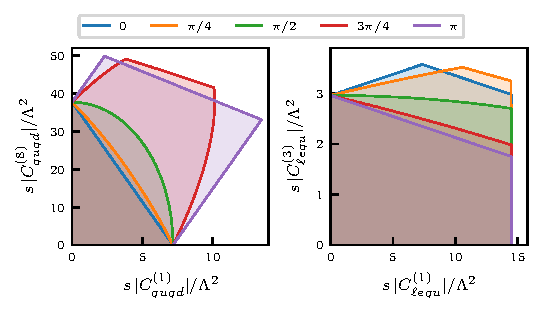
\includegraphics[scale=1.25]{images/C_quqd_and_C_lequ.pdf}
%     \caption{Parameter space allowed by unitarity bounds in the plane of Wilson coefficients in the single-flavor limit.
%     In the two lower plots, we also show the dependence on the relative complex phases $\operatorname{arg}(C_{quqd}^{(1)}/C_{quqd}^{(8)})$ and $\operatorname{arg}(C_{\ell equ}^{(1)}/C_{\ell equ}^{(3)})$.}
%     \label{fig:uni3}
% \end{figure}
\begin{figure}[htbp]
    \centering
    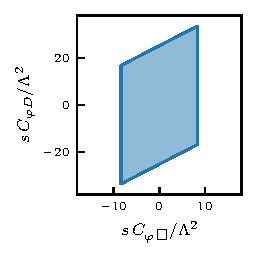
\includegraphics[width=0.25\textwidth]{images/C_H4D2.pdf}\hfill
    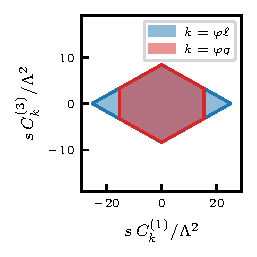
\includegraphics[width=0.25\textwidth]{images/C_Hl_and_C_Hq.pdf}\hfill
    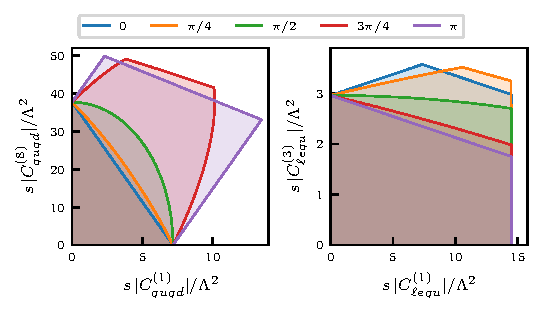
\includegraphics[width=0.48\textwidth]{images/C_quqd_and_C_lequ.pdf}
    \caption{Parameter space allowed by unitarity bounds in the plane of Wilson coefficients in the single-flavor limit.
    In the right-hand panel, we also show the dependence on the relative complex phases $\operatorname{arg}(C_{quqd}^{(1)}/C_{quqd}^{(8)})$ and $\operatorname{arg}(C_{\ell equ}^{(1)}/C_{\ell equ}^{(3)})$.}
    \label{fig:uni3}
\end{figure}

% \begin{figure}[htbp]
%     \centering
%     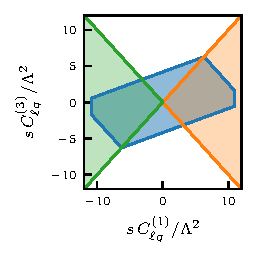
\includegraphics[scale=1.25]{images/C_lq.pdf}\qquad
%     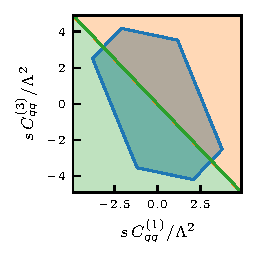
\includegraphics[scale=1.25]{images/C_qq.pdf}\\
%     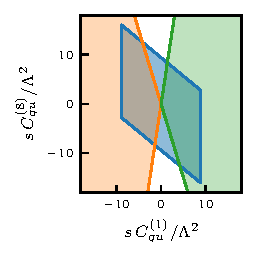
\includegraphics[scale=1.25]{images/C_qu.pdf}\qquad
%     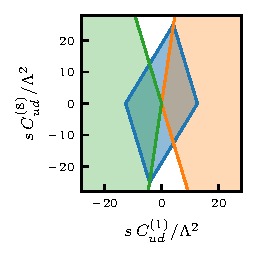
\includegraphics[scale=1.25]{images/C_ud.pdf}
%     \caption{Parameter space allowed by unitarity bounds (blue) and spinning sum rules, discussed in Section~\ref{sec:SMEFT_sumrules}, in the cases of scalar (orange) and vector (green) dominance, 
%     in the single-flavor limit. The missing plot for the Wilson coefficients $C_{qd}^{(1,8)}$ is identical to that of $C_{qu}^{(1,8)}$.}
%     \label{fig:1-flavor unitary+sum rules}
% \end{figure}
\begin{figure}[htbp]
    \centering
    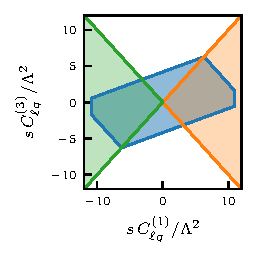
\includegraphics[width=0.25\textwidth]{images/C_lq.pdf}\hfill
    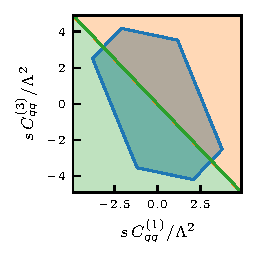
\includegraphics[width=0.25\textwidth]{images/C_qq.pdf}\hfill
    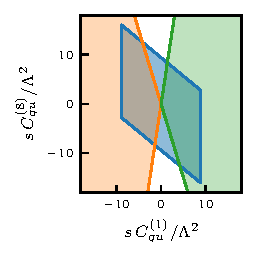
\includegraphics[width=0.25\textwidth]{images/C_qu.pdf}\hfill
    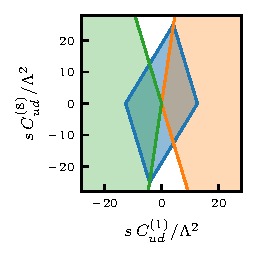
\includegraphics[width=0.25\textwidth]{images/C_ud.pdf}
    \caption{Parameter space allowed by unitarity bounds (blue) and spinning sum rules, discussed in Section~\ref{sec:SMEFT_sumrules}, in the cases of scalar (orange) and vector (green) dominance, 
    in the single-flavor limit. The missing plot for the Wilson coefficients $C_{qd}^{(1,8)}$ is identical to that of $C_{qu}^{(1,8)}$.}
    \label{fig:1-flavor unitary+sum rules}
\end{figure}

To fully exploit the power of this method, we performed a fully coupled-channel analysis
%for each operator. In particular, to compute the amplitude of a process mediated by a given SMEFT operator, we 
%considered all possible initial and final states in all allowed helicity, gauge, and flavor configurations.
by considering all possible initial and final states in all allowed helicity, gauge, and flavor configurations.
At dimension six, the leading numerical constraints often arise from the lowest-multiplicity channels. Nevertheless, the general $N \to M$ formalism of Chapter~\ref{ch:generalizedUB} is essential for a uniform treatment of all operator classes, including $\varphi^6$ and $\psi^2\varphi^3$, and makes the inclusion of higher-multiplicity channels automatic
whenever they yield the leading energy growth.
For practical purposes, we present in Table~\ref{tab:UniBounds} the unitarity bounds assuming single-flavor fermions, due to the large number of independent components arising from Wilson coefficients with multiple flavor indices.
The multi-flavor scenario is considered in Section~\ref{sec:SMEFT_multiflavor}.

The coupled-channel analysis also requires care in the choice of the angular momentum at which the
bound is imposed. 
% For operators containing a single fermionic bilinear, the lowest allowed angular
% momentum in $2\to2$ processes is $J=1/2$, reached through the channels
% \begin{gather}
%     \psi_R^{\alpha,p}\varphi_j\to \psi_L^{i,\beta,r}X^I\,,\qquad \psi_R^{\alpha,p}X^I\to \psi_L^{i,\beta,r}\varphi_j^\dagger\,,\\
%     \psi_R^{\alpha,p}\varphi_i\to\psi_R^{\beta,r}\varphi_j\,,\qquad    \psi_L^{k,\alpha,p}\varphi_i\to\psi_L^{\ell,\beta,r}\varphi_j\,,
% \end{gather}
% where $\alpha,\beta$ are $SU(3)_c$ indices in the (anti)fundamental representation and $L,R$ denote
% the chirality of the fermion fields, while at $J=1$ the additional channels are
% \begin{equation}
%     \psi_R^{\alpha,p}\overline \psi_L^{i,\beta,r}\to X^I\varphi_j^\dagger\,,\qquad \psi_R^{\alpha,p}\overline \psi_R^{\beta,r}\to\varphi_i\varphi_j^\dagger\,, \qquad \psi_L^{k,\alpha,p}\overline \psi_L^{\ell,\beta,r}\to\varphi_i\varphi_j^\dagger\,.
% \end{equation}
Operators containing a single fermionic bilinear generate $2\to2$ processes with
two fermionic and two bosonic external legs. Since a pair of fermions carries integer total angular
momentum, half-integer values of $J$ are reached only when one fermion sits in the initial and one in
the final state, and the lowest allowed value is then $J=1/2$. A minimal set of such channels is
\begin{gather}
    \psi_R^{a,p}\,\varphi^{b} \to \psi_R^{c,r}\,\varphi^{d}\,,\qquad
    \psi_L^{a,p}\,\varphi^{b} \to \psi_L^{c,r}\,\varphi^{d}\,,\qquad
    \psi_R^{a,p}\,\varphi^{b} \to \psi_L^{c,r}\,X^{d}\,,
\end{gather}
where $a,b,c,d$ collectively denote the gauge indices of each field, $p,r$ are flavor
indices, and $L,R$ denote the chirality of the fermions. The first two channels arise from the
chirality-preserving bilinears of the class $\psi^2\varphi^2D$, the third from the
chirality-violating ones of the class $\psi^2X\varphi$. All the remaining $J=1/2$ channels, such as
$\psi_R^{a,p}X^{b}\to\psi_L^{c,r}\varphi^{\dagger d}$, follow from these by applying C, P, T, or
combinations thereof.
Integer values of $J$ instead require both fermions on the same side. For $J=1$, a
minimal set of channels is
\begin{gather}
    \psi_R^{a,p}\,\overline\psi_R^{b,r} \to \varphi^{c}\,\varphi^{\dagger d}\,,\qquad
    \psi_L^{a,p}\,\overline\psi_L^{b,r} \to \varphi^{c}\,\varphi^{\dagger d}\,,\qquad
    \psi_R^{a,p}\,\overline\psi_L^{b,r} \to X^{c}\,\varphi^{\dagger d}\,,
\end{gather}
% where in the first two the chirality-preserving fermion pair already carries one unit of angular
% momentum along the collision axis, while in the third the chirality-violating pair carries none and
% the bound comes instead from the vector in the final state. 
where the minimum $J$ of each pair is set by its helicity difference, which is one unit for
the first two initial states and, in the third, for the final state.
Again, all the remaining channels follow
by applying C, P, T, or combinations thereof.
The resulting bounds are compared in Table~\ref{tab: UB for psi^2 Xphi and psi^2phi^2D}. For
operators of type $\psi^2X\varphi$ the $J=1/2$ bounds are always the stronger ones, whereas for
operators of type $\psi^2\varphi^2D$ the outcome depends on the case at hand, since in the
coupled-channel analysis the color degrees of freedom can add up and make the $J=1$ bound stronger,
even though it would naively be expected to be suppressed.

\begin{table}[tb]
\renewcommand{\arraystretch}{1.4}
\centering
\begin{tabular}{c|cc||c|cc}
\toprule
\rowcolor{hdrcolor}
\boldmath$\psi^2X\varphi$ & \boldmath$J=1/2$ & \boldmath$J=1$
& \boldmath$\psi^2\varphi^2D$ & \boldmath$J=1/2$ & \boldmath$J=1$ \\
\midrule
$C_{eW}$ & $4\pi\sqrt{2/3}$ & $4\pi\sqrt{3}$ 
& $C_{\varphi e}$ & $8\pi$ & $12\pi$ \\
$C_{eB}$ & $4\pi$ & $12\pi$ 
& $C_{\varphi u}$ & $8\pi$ & $4\pi\sqrt{3}$ \\
$C_{uW}$ & $4\pi\sqrt{2/3}$ & $4\pi$ 
& $C_{\varphi d}$ & $8\pi$ & $4\pi\sqrt{3}$ \\
$C_{dW}$ & $4\pi\sqrt{2/3}$ & $4\pi$ 
& $C_{\varphi ud}$ & $8\pi$ & $4\pi\sqrt{6}$ \\
$C_{uB}$ & $4\pi$ & $4\pi\sqrt{3}$ 
& $C_{\varphi \ell}^{(1)}$ & $8\pi$ & $6\pi\sqrt{2}$ \\
$C_{dB}$ & $4\pi$ & $4\pi\sqrt{3}$ 
& $C_{\varphi \ell}^{(3)}$ & $8\pi/3$ & $6\pi\sqrt{2}$ \\
$C_{uG}$ & $2\pi\sqrt{3}$ & $12\pi\sqrt{2}$ 
& $C_{\varphi q}^{(1)}$ & $8\pi$ & $2\pi\sqrt{6}$ \\
$C_{dG}$ & $2\pi\sqrt{3}$ & $12\pi\sqrt{2}$ 
& $C_{\varphi q}^{(3)}$ & $8\pi/3$ & $2\pi\sqrt{6}$ \\
\bottomrule
\end{tabular}
\caption{Comparison of the unitarity bounds on the modulus of the individual Wilson coefficients
associated with the operator classes $\psi^2 X \varphi$ and $\psi^2 \varphi^2 D$, resulting from the
partial waves with $J=1/2$ and $J=1$. The factors $s/\Lambda^2$ are left implicit, as in
Table~\ref{tab:UniBounds}.}
\label{tab: UB for psi^2 Xphi and psi^2phi^2D}
\end{table}


% For four-fermion operators the relevant angular momentum depends strongly on the chirality of the
% external fermions. The channels contributing at $J=0$ are
% \begin{gather}
%     \psi_R^{\alpha,p}\psi_R^{\beta,r}\to\psi_R^{\gamma,s}\psi_R^{\delta,t}\,,\qquad \psi_L^{i,\alpha,p}\psi_L^{j,\beta,r}\to\psi_L^{k,\gamma,s}\psi_L^{\ell,\delta,t}\,,\\
%     \psi_R^{\alpha,p}\psi_R^{\beta,r}\to\psi_L^{i,\gamma,s}\psi_L^{j,\delta,t}\,,\qquad \psi_R^{\alpha,p}\overline\psi_L^{i,\beta,r}\to\psi_R^{\gamma,s}\overline\psi_L^{j,\delta,t}\,,
% \end{gather}
% while those contributing at $J=1$ are
% \begin{gather}
%     \psi_R^{\alpha,p}\overline\psi_R^{\beta,r}\to\psi_R^{\gamma,s}\overline\psi_R^{\delta,t}\,,\qquad \psi_L^{i,\alpha,p}\overline\psi_L^{j,\beta,r}\to\psi_L^{k,\gamma,s}\overline\psi_L^{\ell,\delta,t}\,,\\
%     \psi_R^{\alpha,p}\overline\psi_R^{\beta,r}\to\psi_L^{i,\gamma,s}\overline\psi_L^{j,\delta,t}\,,\qquad \psi_R^{\alpha,p}\psi_L^{i,\beta,r}\to\psi_R^{\gamma,s}\psi_L^{j,\delta,t}\,.
% \end{gather}
For four-fermion operators, the relevant angular momentum is again fixed by the chirality of the
external fermions. A minimal set of channels contributing at $J=0$ is
\begin{gather}
    \psi_R^{a,p}\psi_R^{b,r}\to\psi_R^{c,s}\psi_R^{d,t}\,,\qquad
    \psi_R^{a,p}\psi_R^{b,r}\to\psi_L^{c,s}\psi_L^{d,t}\,,\qquad
    \psi_R^{a,p}\overline\psi_L^{b,r}\to\psi_R^{c,s}\overline\psi_L^{d,t}\,,
\end{gather}
while at $J=1$ it is
\begin{gather}
    \psi_R^{a,p}\overline\psi_R^{b,r}\to\psi_R^{c,s}\overline\psi_R^{d,t}\,,\qquad
    \psi_R^{a,p}\overline\psi_R^{b,r}\to\psi_L^{c,s}\overline\psi_L^{d,t}\,,\qquad
    \psi_R^{a,p}\psi_L^{b,r}\to\psi_R^{c,s}\psi_L^{d,t}\,.
\end{gather}
All the remaining channels follow by applying C, P, T, or
combinations thereof.
The corresponding bounds are compared in Table~\ref{tab: UB for psi^4}. In most cases, the $J=0$ bound
dominates, but not always, which stresses once again that, to obtain the most stringent bounds, one cannot stop at the smallest allowed
angular momentum whenever several degrees of freedom contribute to the coupled-channel analysis.

\begin{table}[htbp]
\renewcommand{\arraystretch}{1.4}
\centering
\begin{tabular}{c|cc||c|cc}
\toprule
\rowcolor{hdrcolor}
\boldmath$(\overline L L)(\overline L L)$ & \boldmath$J=0$ & \boldmath$J=1$
& {\boldmath$(\overline{L}R)(\overline{R}L)$}/{\boldmath$(\overline{L}R)(\overline{L}R)$} & \boldmath$J=0$ & \boldmath$J=1$ \\
\midrule
$C_{\ell\ell}$ & $2\pi$ & $2\pi$ 
& $C_{\ell e d q}$ & $8\pi/\sqrt{3}$ & $24\pi$ \\
$C_{qq}^{(1)}$ & $2\pi$ & $6\pi/7$ 
& $C_{quqd}^{(1)}$ & $16\pi/7$ & $24\pi$ \\
$C_{qq}^{(3)}$ & $2\pi$ & $6\pi/5$ 
& $C_{quqd}^{(8)}$ & $12\pi$ & $36\pi$ \\
$C_{\ell q}^{(1)}$ & $4\pi$ & $2\pi\sqrt{3}$ 
& $C_{\ell equ}^{(1)}$ & $8\pi/\sqrt{3}$ & $24\pi\sqrt{2}$ \\
$C_{\ell q}^{(3)}$ & $4\pi/3$ & $2\pi\sqrt{3}$ 
& $C_{\ell e qu}^{(3)}$ & $2\pi\sqrt{2}/3$ & $2\pi\sqrt{3}$ \\
\midrule
\rowcolor{hdrcolor}
\boldmath$(\overline RR)(\overline RR)$ & \boldmath$J=0$ & \boldmath$J=1$
& \boldmath$(\overline L L)(\overline R R)$ & \boldmath$J=0$ & \boldmath$J=1$ \\
\midrule
$C_{ee}$ & $2\pi$ & $3\pi$ 
& $C_{\ell e}$ & $4\pi$ & $6\pi\sqrt{2}$ \\
$C_{uu}$ & $2\pi$ & $3\pi/2$ 
& $C_{\ell u}$ & $4\pi$ & $2\pi\sqrt{6}$ \\
$C_{dd}$ & $2\pi$ & $3\pi/2$ 
& $C_{\ell d}$ & $4\pi$ & $2\pi\sqrt{6}$ \\
$C_{eu}$ & $4\pi$ & $4\pi\sqrt{3}$ 
& $C_{qe}$ & $4\pi$ & $2\pi\sqrt{6}$ \\
$C_{ed}$ & $4\pi$ & $4\pi\sqrt{3}$ 
& $C_{qu}^{(1)}$ & $4\pi$ & $2\pi\sqrt{2}$ \\
$C_{ud}^{(1)}$ & $4\pi$ & $4\pi$ 
& $C_{qu}^{(8)}$ & $3\pi$ & $12\pi\sqrt{2}$ \\
$C_{ud}^{(8)}$ & $6\pi$ & $9\pi$ 
& $C_{qd}^{(1)}$ & $4\pi$ & $2\pi\sqrt{2}$ \\
& & & $C_{qd}^{(8)}$ & $3\pi$ & $12\pi\sqrt{2}$ \\
\bottomrule
\end{tabular}
\caption{Comparison of the unitarity bounds on the modulus of the individual Wilson coefficients
associated with the four-fermion operators, resulting from the partial waves with $J=0$ and $J=1$.
The factors $s/\Lambda^2$ are left implicit, as in Table~\ref{tab:UniBounds}.}
\label{tab: UB for psi^4}
\end{table}


Lastly, for operators of the type $X^3$ involving three gauge field strengths, the unitarity bounds were computed using amplitudes that include both the SM contribution and at most one SMEFT insertion, effectively truncating the calculation at $\mathcal{O}(1/\Lambda^2)$ at the amplitude level. 
Contributions of order $1/\Lambda^4$ could, in principle, yield stronger bounds, especially when the gauge coupling is small; however, including them without simultaneously accounting for dimension-eight operators would be inconsistent.
Indeed, from positivity constraints, the presence of a dimension-six operator of type $X^3$ necessarily implies the existence of a dimension-eight operator of type $X^4$, which would inevitably affect the resulting unitarity bounds; see Ref.~\cite{Ghosh:2022qqq}.

Comparing the results in Table \ref{tab:UniBounds} with previous SMEFT analyses \cite{Corbett:2014ora,Corbett:2017qgl,Cao:2023qks}, we derive unitarity bounds for the complete set of four-fermion operators and for operators involving at least one gluon field, which were not covered in those works.
With this method, such bounds are straightforward to obtain compared to alternative approaches. Moreover, the fully exploited coupled-channel analysis allows us to derive stronger bounds than those previously reported. 

Overall, our bounds on purely bosonic operators agree with those in Ref.~\cite{Cao:2023qks}, except for a factor-of-two difference arising from Eq.~\eqref{unitarity bound general}, as that work conventionally imposed $|a_{i\to f}^J|\leq 2$ for the partial-wave coefficients. In contrast, the bounds on operators involving fermions exhibit larger discrepancies, which we attribute to the combined effects of the coupled-channel analysis and the marginalization procedure. In particular, operators of the type $\psi^2 X\varphi$ and $\psi^2\varphi^2 D$ show case-by-case differences of up to a factor of two. Overall, our bounds are always more stringent, except for $O_{\varphi ud}$, for which our bound is weaker by a factor of $\sqrt{2}$.

\section{Spinning Sum-Rule Bounds\label{sec:SMEFT_sumrules}}

As anticipated in the introduction, the analyticity of the $S$-matrix, together with partial-wave
unitarity, yields additional constraints on effective four-fermion interactions. The relevant
dispersion relations have been introduced in
Refs.~\cite{Low:2009di,Azatov:2021ygj,Gu:2020thj,Remmen:2020uze,Remmen:2022orj,Altmannshofer:2023bfk,%
Altmannshofer:2025lun}, and we derive here the resulting inequalities in the Warsaw basis.

% Following Ref.~\cite{Remmen:2020uze}, we consider the amplitude $\mathcal{A}_{\alpha\beta}(s,t)$,
% where $s$ and $t$ are the usual Mandelstam variables associated with an elastic scattering process of
% two fermions whose quantum numbers, such as flavor and helicity, are collectively denoted by $\alpha$
% and $\beta$. Expanding the UV amplitude in partial waves of fixed total angular momentum,
% $a_{\alpha\beta}^{J}(s)$, one finds\footnote{Note that our partial-wave coefficients are normalized
% differently from those of Ref.~\cite{Remmen:2020uze}.}
Following Ref.~\cite{Remmen:2020uze}, we consider the amplitude $\mathcal{A}_{\alpha\beta}(s,t)$,
where $s$ and $t$ are the usual Mandelstam variables associated with the elastic scattering of two
fermions of opposite helicity, whose internal quantum numbers, such as flavor and gauge charges, are
collectively denoted by $\alpha$ and $\beta$. We write $\overline\alpha$ for the state obtained by
crossing, with conjugated quantum numbers and reversed helicity. The initial state then carries one
unit of net helicity, so that its partial-wave expansion starts at $J=1$, whereas the crossed one has
vanishing net helicity and starts at $J=0$. Expanding the UV amplitude in partial waves of fixed
total angular momentum, $a_{\alpha\beta}^{J}(s)$, one finds\footnote{Note that our partial-wave coefficients are normalized
differently from those of Ref.~\cite{Remmen:2020uze}.}
\begin{multline}\label{eq: sum rules with boundary}
        \lim_{s\to 0}\partial_s\mathcal{A}_{\alpha\beta}(s,0)+C_{\alpha\beta}^{(s,\infty)}=-\lim_{s\to 0}\partial_s\mathcal{A}_{\overline \alpha\beta}(s,0)-C_{\overline\alpha\beta}^{(s,\infty)} \\
        =8\int_{s_0}^\infty \frac{\dd s}{s^2}\left[-\Im a_{\overline{\alpha}\beta}^{0}(s)+\sum_{J=1}^\infty(2J+1)\left(\Im a_{\alpha\beta}^{J}(s)-\Im a_{\overline{\alpha}\beta}^{J}(s)\right)\right]\,,
\end{multline}
where $s_0$ is the characteristic mass-squared scale of the UV completion and the boundary term is
defined as
\begin{equation}
    C_{\alpha\beta}^{(s,\infty)}=\Res_{s=\infty}\frac{\mathcal{A}_{\alpha\beta}(s,0)}{s^2}=-\lim_{\abs{s}\to \infty}\frac{\mathcal{A}_{\alpha\beta}(s,0)}{s}\,.
\end{equation}
The same contour argument applied to the coefficient of $t$ in $\mathcal{A}_{\alpha\beta}(0,t)$
yields a second, beyond-forward dispersion relation, with its own boundary term
$C^{(t,\infty)}_{\alpha\beta}$. Since the dimension-six amplitude of two opposite-helicity fermions
is proportional to $[13]\langle 24\rangle$, the sum of the two relations has a vanishing left-hand
side up to boundary terms, while on the right-hand side every partial wave enters with a
non-negative weight. If all boundary terms vanish and the partial-wave expansion converges, each
contribution must then vanish separately, so that $\Im a_{\alpha\beta}^{J}$ and
$\Im a_{\overline\alpha\beta}^{J}$ vanish for every $J\geq2$, together with
$\Im a_{\overline\alpha\beta}^{1}$. Only a scalar and a vector channel are left, and
Eq.~\eqref{eq: sum rules with boundary} reduces to~\cite{Remmen:2020uze}
\begin{equation}\label{eq: sum rules master equation}
    \lim_{s\to 0}\partial_s\mathcal{A}_{\overline \alpha\beta}(s,0) = -\lim_{s\to 0}\partial_s\mathcal{A}_{ \alpha\beta}(s,0) =8\int_{s_0}^\infty \frac{\dd s}{s^2}\left(\Im a_{\overline{\alpha}\beta}^{0}(s)-3\Im a_{\alpha\beta}^{1}(s)\right)\,.
\end{equation}
Dominance of spin-0 (spin-1) states in the UV theory implies that the left-hand side of
Eq.~\eqref{eq: sum rules master equation} is positive (negative) definite for any choice of $\alpha$
and $\beta$. This property can be exploited to derive constraints among the flavor-dependent entries
of the Wilson coefficients of four-fermion SMEFT operators, or between different $\psi^4$ operators
with the same fermionic content. Since Ref.~\cite{Remmen:2020uze} adopts a basis different from the
Warsaw one, we report the corresponding combinations in Table~\ref{tab:sum_rules}. When contracted
with $\alpha_p \alpha_r^* \beta^*_s \beta_t$, they are positive (negative) if the completion is
dominated by scalars (vectors).
%
\begin{table}[h!t!b!]
\renewcommand{\arraystretch}{1.5}
    \centering
    \begin{tabular}{cc}
    \toprule
    \rowcolor{hdrcolor}
    \textbf{Operator class} & \textbf{Spinning sum rules} \\
    \midrule
    \multirow{6}{*}{\boldmath$(\overline{R}R)(\overline{R}R)$} &
    $[C_{ee}]_{prst}$ \\
    & $[C_{uu}]_{prst}$\,, \qquad $[C_{uu}]_{prst} + [C_{uu}]_{ptsr}$ \\
    & $[C_{dd}]_{prst}$\,, \qquad $[C_{dd}]_{prst} + [C_{dd}]_{ptsr}$ \\
    & $[C_{eu}]_{prst}$\,, \qquad $[C_{ed}]_{prst}$ \\
    & $[C_{ud}^{(1)}]_{prst}+\tfrac{1}{4}[C_{ud}^{(8)}]_{prst}$ \\
    & $[C_{ud}^{(1)}]_{prst}-\tfrac{1}{6}[C_{ud}^{(8)}]_{prst}$ \\
    \midrule
    \multirow{5}{*}{\boldmath$(\overline{L}L)(\overline{L}L)$} &
    $[C_{\ell\ell}]_{prst}$\,, \qquad $[C_{\ell\ell}]_{prst} + [C_{\ell\ell}]_{ptsr}$ \\
    & $[C_{qq}^{(1)}]_{prst} + [C_{qq}^{(1)}]_{ptsr} + [C_{qq}^{(3)}]_{prst} + [C_{qq}^{(3)}]_{ptsr}$ \\
    & $[C_{qq}^{(1)}]_{prst} - [C_{qq}^{(3)}]_{prst} + 2[C_{qq}^{(3)}]_{ptsr}$ \\
    & $[C_{\ell q}^{(1)}]_{prst} + [C_{\ell q}^{(3)}]_{prst}$ \\
    & $[C_{\ell q}^{(1)}]_{prst} - [C_{\ell q}^{(3)}]_{prst}$ \\
    \midrule
    \multirow{6}{*}{\boldmath$(\overline{L}L)(\overline{R}R)$} &
    $-[C_{\ell e}]_{prst}$\,, \qquad $-[C_{\ell u}]_{prst}$ \\
    & $-[C_{\ell d}]_{prst}$\,, \qquad $-[C_{qe}]_{prst}$ \\
    & $-[C_{qu}^{(1)}]_{prst} - \tfrac{1}{4}[C_{qu}^{(8)}]_{prst}$ \\
    & $-[C_{qu}^{(1)}]_{prst} + \tfrac{1}{6}[C_{qu}^{(8)}]_{prst}$ \\
    & $-[C_{qd}^{(1)}]_{prst} - \tfrac{1}{4}[C_{qd}^{(8)}]_{prst}$ \\
    & $-[C_{qd}^{(1)}]_{prst} + \tfrac{1}{6}[C_{qd}^{(8)}]_{prst}$ \\
    \bottomrule
    \end{tabular}
    \caption{Combinations of four-fermion Wilson coefficients that, when contracted with $\alpha_p \alpha_r^* \beta^*_s \beta_t$, are positive (negative) if the UV completion is dominated by scalars (vectors).}
    \label{tab:sum_rules}
\end{table}
%

% Sum rules can in principle be derived for all dimension-six SMEFT Wilson coefficients. They depend,
% however, on the superposition of field states encoded in the vectors $\alpha$ and $\beta$, so that,
% even when the boundary terms vanish, they do not translate into a definite sign of the Wilson
% coefficients, unlike what happens for $\psi^4$ operators.
% For purely bosonic operators the boundary
% terms are generically present and depend on the $SU(2)_L$ configuration, so that no robust
% information can be extracted. For $\psi^2\varphi^2D$ operators one has to fix a configuration for the
% Higgs fields, after which no information is left for the flavor indices, since no spinning sum rules
% arise there~\cite{Remmen:2022orj}.

Spinning sum rules are not confined to four-fermion operators, but only for the latter do they
translate into a definite sign of a Wilson coefficient. For the purely bosonic operators of the class
$\varphi^4 D^2$, they can still be constructed, although only for a restricted cone of combinations of the
corresponding coefficients, and with the correlation between sign and spin reversed with respect to
the fermionic case~\cite{Remmen:2022orj}. For operators involving gauge bosons, the boundary terms are
generically present and depend on the $SU(2)_L$ configuration, so that the sum rules are of
indefinite sign. What survives is the sharper statement that, if the boundary terms vanish, the UV
amplitudes mediating elastic vector scattering must vanish identically~\cite{Remmen:2022orj}. For
$\psi^2\varphi^2D$ operators, one has to fix a configuration for the Higgs fields, and no spinning sum
rule arises. The dispersion relations remain informative --- vanishing boundary terms force the UV to
be dominated by a fermionic mode --- but they no longer discriminate between scalar and vector
dominance~\cite{Remmen:2022orj}.


As an illustration, Figure~\ref{fig:1-flavor unitary+sum rules} shows the parameter space allowed by
the unitarity bounds and by the spinning sum rules under scalar and vector dominance for four-fermion
Wilson coefficients in the single-flavor limit. Stronger bounds generally arise in the three-flavor
scenario, which is the subject of Section~\ref{sec:SMEFT_multiflavor}.

\subsection{Application}

We now describe how the sum rules associated with a given four-fermion operator are turned into
inequalities on its Wilson coefficients. For scalar dominance one has to impose
\begin{equation}
    b^\psi_{prst}\,\alpha_p \alpha_r^* \beta^*_s \beta_t\geq0\qquad \forall\,\alpha,\beta\,,
\end{equation}
where $\alpha,\beta$ are complex three-vectors in flavor space and $b_{prst}^\psi$ are the
combinations of Table~\ref{tab:sum_rules}. This is a double quadratic form in $\alpha$ and $\beta$.
We therefore first impose the inequality for every $\alpha$, which amounts to a quadratic form, by
introducing the $3\times 3$ matrices
\begin{equation}
    M^\psi_{pr}= b^\psi_{prst}\,\beta^*_s \beta_t
\end{equation}
and requiring all their eigenvalues to be non-negative for every $\beta$. Without loss of generality, we
parameterize
\begin{equation}
    \beta=
    \begin{pmatrix}
        e^{i\delta_1}\beta_1 \\ e^{i\delta_2}\beta_2 \\ \sqrt{1-\beta_1^2-\beta_2^2}
    \end{pmatrix}\,,
\end{equation}
% so that the eigenvalues of $M^\psi$ always take the form
% \begin{equation}\label{eq:eigenvalue form}
%     f(x)=a + bx - \sqrt{c^2 + dx + ex^2}\,,\qquad x=\beta_3^2\,,
% \end{equation}
and in all the cases encountered, the eigenvalues of $M^\psi$ take the form
\begin{equation}\label{eq:eigenvalue form}
    f_\pm(x)=a + bx \pm \sqrt{c^2 + dx + ex^2}\,,\qquad x=\beta_1^2+\beta^2_2\,,
\end{equation}
with $a,b,c,d,e\in\mathbb{R}$.
Requiring all eigenvalues to be positive for
every $\beta$ is therefore equivalent to requiring $f_-(x)\geq0$ for every $x\in[0,1]$.

% This last step is what makes the procedure practicable. 
Scanning numerically over $\beta$ would give
only a sampled, and therefore inconclusive, version of the constraint, whereas the positivity of $f_-$
on the unit interval can be traded for a finite set of algebraic inequalities among the coefficients
$a,b,c,d,e$, which are themselves functions of the Wilson coefficients. Explicitly, $f_-(x)\geq0$ for
every $x\in[0,1]$ if and only if
\begin{align}\label{eq:Delta}
    \Delta(a,b,c,d,e) &= 
    a \ge 0 
    \ \land \
    a+b \ge 0
    \ \land \ 
    a^2 - c^2 \ge 0
    \ \land \ 
    (a+b)^2 - c^2 -d-e \ge 0 \nonumber
    \\& \quad
    \land \
    [e - b^2 \ge 0 \ \lor\  (2ab-d)(2ab-d+2b^2-2e) \ge 0 \nonumber 
    \\& \quad
    \lor \ 4(b^2-e)(a^2-c^2)-(2ab-d)^2 \ge 0]
\end{align}
holds, as proved in Appendix~\ref{sec:appendix, logical expression}.
For vector dominance one follows the same steps, requiring instead all eigenvalues to be non-positive.

\subsection{Limitations}

Unlike the partial-wave unitarity bounds, which follow solely from the consistency of the EFT, the
spinning sum rules are considerably more model dependent and hold only under a specific set of
assumptions whose violation invalidates the corresponding
inequalities~\cite{Remmen:2020uze,Remmen:2022orj,Azatov:2021ygj,Gu:2020thj}. In particular:
\begin{itemize}
    \item They assume tree-level UV completions and can be violated at loop level~\cite{Azatov:2021ygj,Remmen:2020uze};
    \item They assume dominance by states of definite spin, so that completions involving a
    non-trivial interplay of spin-0 and spin-1 states can evade them, since the right-hand side of
    Eq.~\eqref{eq: sum rules master equation} ceases to be sign definite for arbitrary configurations
    of $\alpha$ and $\beta$;
    \item They rely on the vanishing of the boundary terms in the dispersion relation, which fails in
    particular for vector $t$-channel UV
    completions~\cite{Remmen:2020uze,Remmen:2022orj,Azatov:2021ygj}.
\end{itemize}
% The last condition is the most problematic one, since tree-level UV completions of $\psi^4$
% operators generically arise in new-physics models.
The last condition is the most restrictive one in practice, since $t$-channel vector mediators of
four-fermion operators arise generically in new-physics models.

This residual model dependence is, however, physically informative. A coefficient lying outside the
scalar- and vector-dominated regions does not exclude a UV completion but points to a more
structured one, such as a vector $t$-channel mediator, a loop-level origin, or a mixed-spin spectrum.
In Appendix~\ref{app:SMEFT_UV} we verify this picture explicitly by matching a representative set of
tree-level UV completions of Ref.~\cite{deBlas:2017xtg}. All the scalar completions considered there satisfy the
sum-rule constraints, whereas vector $t$-channel completions can violate them.

\section{Bounds on Flavorful Four-Fermion Operators\label{sec:SMEFT_multiflavor}}

The results presented so far assume a single fermion flavor. In the SMEFT, the basis of $\psi^4$
operators accounts for thousands of independent coefficients once the full flavor structure of the SM
fermions is turned on. Specific hypotheses about the symmetries and the symmetry breaking in the
flavor sector therefore play an important role in addressing the question of what information can be
extracted from the theoretical bounds derived above. The drawback is that this necessarily introduces
some model dependence. Still, reasonable flavor hypotheses have been proposed in the literature and
used in many beyond-the-SM studies, precisely in order to deal with the proliferation of independent
$\psi^4$ Wilson coefficients.

\subsection{Flavor Symmetries}

Historically, the most widely adopted hypothesis is Minimal Flavor Violation (MFV), first introduced
in Ref.~\cite{DAmbrosio:2002vsn} for the quark sector and subsequently extended to the
leptons~\cite{Cirigliano:2005ck}. It assumes that the SM fermions are charged under the global flavor
symmetry group
\begin{equation}
    G_{\rm MFV}\equiv U(3)^5=U(3)_q\times U(3)_u\times U(3)_d\times U(3)_\ell\times U(3)_e\,,
\end{equation}
where each SM fermion is a three-vector in flavor space transforming in the fundamental
representation of one of these factors,
\begin{equation}
    q\to U_q\, q\,,\quad \ell\to U_\ell\, \ell\,,\quad u\to U_u\, u\,,\quad d\to U_d\, d\,,\quad e\to U_e\, e\,.
\end{equation}
The only interactions in the SM Lagrangian that explicitly break $G_{\rm MFV}$ are the Yukawa
matrices $Y_u$, $Y_d$ and $Y_e$, which are promoted to spurions transforming as
\begin{equation}
    Y_u\to U_q Y_u U_u^\dagger\,,\quad Y_d\to U_q Y_d U_d^\dagger\,,\quad Y_e\to U_\ell Y_e U_e^\dagger\,.
\end{equation}
Assuming that new physics also respects $G_{\rm MFV}$, the number of independent coefficients in
four-fermion operators is strongly reduced, since $U(3)^5$-violating terms can arise only through
appropriate Yukawa insertions in the Wilson coefficients, weighted by unknown $\mathcal O(1)$
numbers. The classification of the independent structures arising at dimension six was carried out in
Ref.~\cite{Faroughy:2020ina}. Furthermore, since all the entries of the Yukawa matrices are nearly
vanishing except $[Y_u]_{33}\approx y_t\approx 1$, we neglect all the flavor structures involving
insertions of $Y_d$ or $Y_e$ and retain only the exact structures together with those up to
$\mathcal O(Y_u^2)$.\footnote{In principle, since $y_t\approx1$, an arbitrary number of $Y_u$
insertions should be considered, but this would amount to an effective breaking $U(3)_q\times U(3)_u\to
U(2)_q\times U(2)_u$. We stop at $\mathcal{O}(Y_u^2)$.} In this way the independent coefficients of
$\psi^4$ operators are reduced from $\mathcal O(1000)$ to $\mathcal O(10)$.

Another theoretically motivated hypothesis assumes that the first two generations of each fermion
species transform collectively as doublets while the third generation is a singlet. The flavor
symmetry is then
\begin{equation}
    G_{\rm F}\equiv U(2)^5=U(2)_q\times U(2)_u\times U(2)_d\times U(2)_\ell\times U(2)_e\,,
\end{equation}
where the fermion fields decompose as $\psi = (\psi_a,\psi_3)$, with $a=1,2$ and
$\psi=q,u,d,\ell,e$. The classification of the independent structures at dimension six was again
carried out in Ref.~\cite{Faroughy:2020ina}. In this case there is no unique or well-motivated choice
of spurions parameterizing the breaking of the symmetry~\cite{Faroughy:2020ina,Greljo:2022cah}, but
they are always expected to be small, so that we retain only the exact flavor structures. The number
of independent coefficients of $\psi^4$ operators is again reduced from $\mathcal O(1000)$ to
$\mathcal O(10)$.

In the following we make the symmetrization of the Wilson coefficients explicit, since the bounds
require computing eigenvalues of quadratic forms. For operators built from a single fermion species
we use
\begin{equation}
    [C_{\psi\psi}]_{prst}=[C_{\psi\psi}]_{stpr}=[C_{\psi\psi}]^*_{rpts}\,,
\end{equation}
while for different fermion types
\begin{equation}
    [C_{\psi\chi}]_{prst}=[C_{\psi\chi}]^*_{rpts}\,.
\end{equation}

\subsection{\texorpdfstring{Example: $O_{\ell q}^{(1)}$ and $O_{\ell q}^{(3)}$}{Example: Olq(1) and Olq(3)}}

Under these flavor hypotheses we are able to provide unitarity bounds for the SMEFT Wilson
coefficients involving fermionic fields in the multi-flavor case. As a representative example, we
discuss here the operators $O_{\ell q}^{(1,3)}$. Under MFV each of them admits two independent
coefficients,
\begin{equation}
    [C_{\ell q}^{(i)}]_{prst} = C_{\ell q}^{(i,1)}\delta_{pr}\delta_{st}
    + C_{\ell q}^{(i,2)}\delta_{pr}(Y_u Y_u^\dagger)_{st}\,,\qquad i=1,3\,,
\end{equation}
while under $U(2)^5$ the independent structures are four for each $i$. The corresponding marginalized
bounds are collected in Table~\ref{tab:Olq_UB}, and the allowed regions are shown in
Figures~\ref{fig:Olq_mfv} and \ref{fig:Olq_u2} as two-dimensional slices, in which the remaining
independent coefficients are set to zero.

\begin{table}[htbp]
\centering
{\small
% ---- info block ----
\begin{tabular}{ll}
    \textbf{Operators:} &
        $\boxed{O_{\ell q}^{(1)} = (\overline\ell_p \gamma^\mu \ell_r)(\overline q_s \gamma_\mu q_t),\quad O_{\ell q}^{(3)} = (\overline\ell_p \gamma^\mu \sigma^I \ell_r)(\overline q_s \gamma_\mu \sigma^I q_t)}$ \\[0.2cm]
    \textbf{MFV decomposition:} &
        $[C_{\ell q}^{(i)}]_{prst} =
            C_{\ell q}^{(i,1)}\delta_{pr}\delta_{st}
            + C_{\ell q}^{(i,2)}\delta_{pr}(Y_u Y_u^\dagger)_{st}$,\quad $i=1,3$ \\[0.15cm]
    \textbf{$U(2)^5$ decomposition:} &
        $[C_{\ell q}^{(i)}]_{prst} =
            C_{\ell q}^{(i,1)}\Pij{p}{r}{a}\Pij{s}{t}{b}
            + C_{\ell q}^{(i,2)}\delta_{p3}\delta_{3r}\Pij{s}{t}{a}
            $ \\
        & $\phantom{[C_{\ell q}^{(i)}]_{prst} ={}}+ C_{\ell q}^{(i,3)}\Pij{p}{r}{a}\delta_{s3}\delta_{3t}
            + C_{\ell q}^{(i,4)}\delta_{p3}\delta_{3r}\delta_{s3}\delta_{3t}$,\quad $i=1,3$ \\
\end{tabular}
\\[0.3cm]
% ---- bounds table ----
\renewcommand{\arraystretch}{1.3}
\begin{tabular}{ccccc}
    \toprule
    \rowcolor{hdrcolor}
    \textbf{Symmetry} & \textbf{Coefficient}
        & \textbf{Unitarity bound}
        & \textbf{Scalar dominance}
        & \textbf{Vector dominance} \\
    \midrule
    % --- MFV section ---
    %\rowcolor{seccolor}
    %\multicolumn{5}{l}{\textit{Minimal Flavor Violation}} \\
    \multirow{4}{*}{MFV}
        & $C_{\ell q}^{(1,1)}$ & $[-4.44,\, 4.44]$ & $[0,\, 4.44]$      & $[-4.44,\, 0]$    \\
        & $C_{\ell q}^{(1,2)}$ & $[-7.70,\, 7.70]$ & $[-4.44,\, 6.28]$  & $[-6.28,\, 4.44]$ \\
        & $C_{\ell q}^{(3,1)}$ & $[-4.44,\, 4.44]$ & $[-3.14,\, 4.44]$  & $[-4.44,\, 3.14]$ \\
        & $C_{\ell q}^{(3,2)}$ & $[-7.70,\, 7.70]$ & $[-6.99,\, 7.70]$  & $[-7.70,\, 6.99]$ \\
    \midrule
    % --- U(2)^5 section ---
    %\rowcolor{seccolor}
    %\multicolumn{5}{l}{\textit{$U(2)^5$ Flavor Symmetry}} \\
    \multirow{8}{*}{$U(2)^5$}
        & $C_{\ell q}^{(1,1)}$ & $[-5.44,\, 5.44]$ & $[0,\, 5.44]$      & $[-5.44,\, 0]$    \\
        & $C_{\ell q}^{(1,2)}$ & $[-7.70,\, 7.70]$ & $[0,\, 7.70]$      & $[-7.70,\, 0]$    \\
        & $C_{\ell q}^{(1,3)}$ & $[-7.70,\, 7.70]$ & $[0,\, 7.70]$      & $[-7.70,\, 0]$    \\
        & $C_{\ell q}^{(1,4)}$ & $[-10.9,\, 10.9]$ & $[0,\, 10.9]$      & $[-10.9,\, 0]$    \\
        & $C_{\ell q}^{(3,1)}$ & $[-5.44,\, 5.44]$ & $[-3.14,\, 5.44]$  & $[-5.44,\, 3.14]$ \\
        & $C_{\ell q}^{(3,2)}$ & $[-6.28,\, 6.28]$ & $[-3.14,\, 6.28]$  & $[-6.28,\, 3.14]$ \\
        & $C_{\ell q}^{(3,3)}$ & $[-6.28,\, 6.28]$ & $[-3.14,\, 6.28]$  & $[-6.28,\, 3.14]$ \\
        & $C_{\ell q}^{(3,4)}$ & $[-6.28,\, 6.28]$ & $[-3.14,\, 6.28]$  & $[-6.28,\, 3.14]$ \\
    \bottomrule
\end{tabular}}
\caption{Marginalized partial-wave unitarity bounds for $O_{\ell q}^{(1,3)}$ under MFV and $U(2)^5$
flavor symmetry, with and without spinning sum rules under scalar or vector dominance in the UV.
Bounds are intervals $[a,b]$ with $(s/\Lambda^2)C \in [a,b]$, rounded to 3 significant digits.}
\label{tab:Olq_UB}
\end{table}


\begin{figure}[htbp]
    \centering
    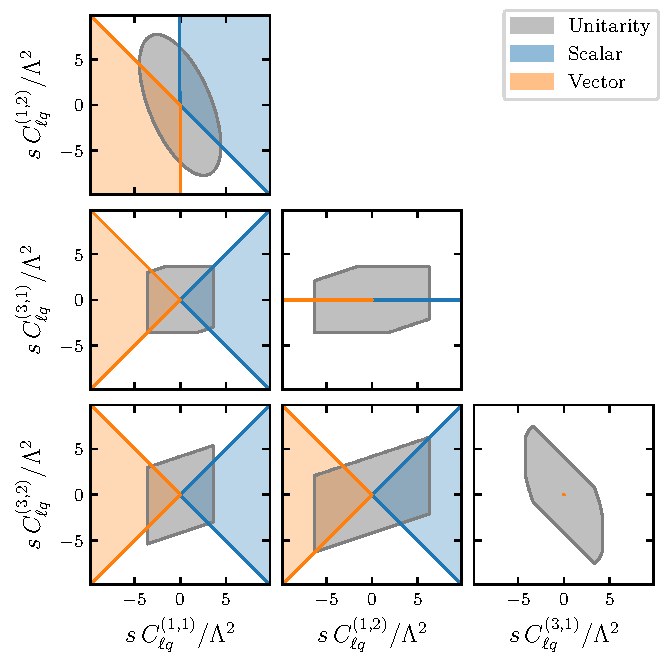
\includegraphics[scale = 0.75]{images/flavor/Olq_mfv.pdf}
    \caption{Partial-wave unitarity bounds and sum-rule constraints (under scalar and vector dominance) for the operators $O_{\ell q}^{(1,3)}$ under MFV, where $[C_{\ell q}^{(i)}]_{prst} =
            C_{\ell q}^{(i,1)}\delta_{pr}\delta_{st}
            + C_{\ell q}^{(i,2)}\delta_{pr}(Y_u Y_u^\dagger)_{st}$, $i=1,3$. The regions shown are two-dimensional slices of the full allowed region, obtained by setting to zero all the independent coefficients other than the two displayed.}
    \label{fig:Olq_mfv}
\end{figure}

\begin{figure}[htbp]
    \centering
    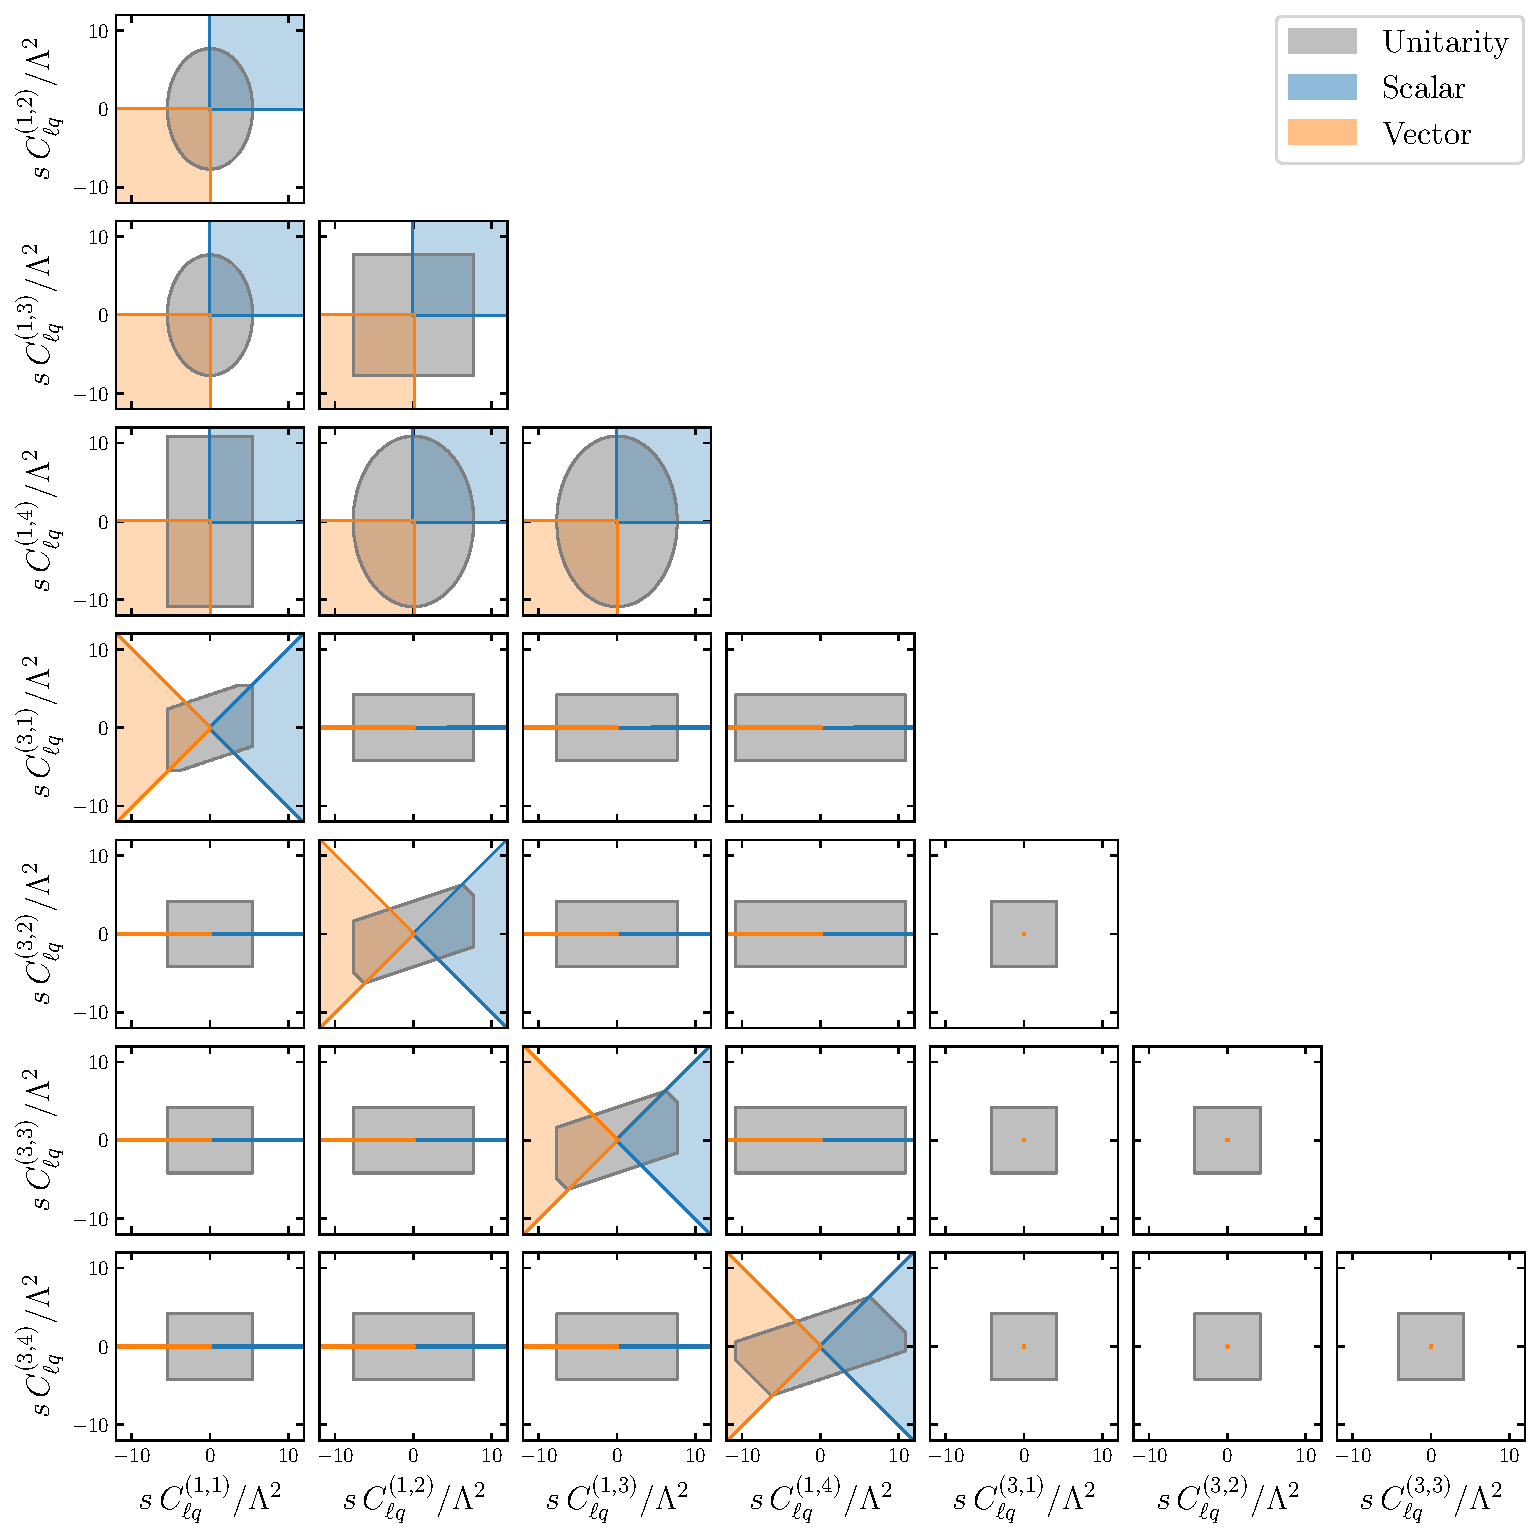
\includegraphics[width=1\linewidth]{images/flavor/Olq_u2.pdf}
    \caption{Partial-wave unitarity bounds and sum-rule constraints (under scalar and vector dominance) for the operators $O_{\ell q}^{(1,3)}$ under $U(2)^5$ flavor symmetry, where $[C_{\ell q}^{(i)}]_{prst} =
            C_{\ell q}^{(i,1)}\Pij{p}{r}{a}\Pij{s}{t}{b}
            + C_{\ell q}^{(i,2)}\delta_{p3}\delta_{3r}\Pij{s}{t}{a}
            + C_{\ell q}^{(i,3)}\Pij{p}{r}{a}\delta_{s3}\delta_{3t}
            + C_{\ell q}^{(i,4)}\delta_{p3}\delta_{3r}\delta_{s3}\delta_{3t}$, $i=1,3$. The regions shown are two-dimensional slices of the full allowed region, obtained by setting to zero all the independent coefficients other than the two displayed.}
    \label{fig:Olq_u2}
\end{figure}


Interestingly, one can notice that setting some coefficients to zero forces the other coefficients to vanish as well in order to satisfy the sum-rule constraints.
This can be seen, e.g., in two panels of Figure~\ref{fig:Olq_mfv} and eighteen panels of Figure~\ref{fig:Olq_u2}, where the sum-rule regions collapse to lines or points.

Even under these flavor hypotheses, the coupled-channel analysis remains demanding. As an illustration,
Figure~\ref{fig:matrixplot} shows the structure of the scattering matrix --- whose
eigenvalues were obtained analytically with finite-field methods~\cite{Chestnov:2025svg} --- associated with the
$q\overline q \to q \overline q$ processes in the three-flavor $U(2)^5$ scenario, considered for obtaining the bounds associated with $O_{qq}^{(1,3)}$.
%
\begin{figure}[htbp]
    \centering
    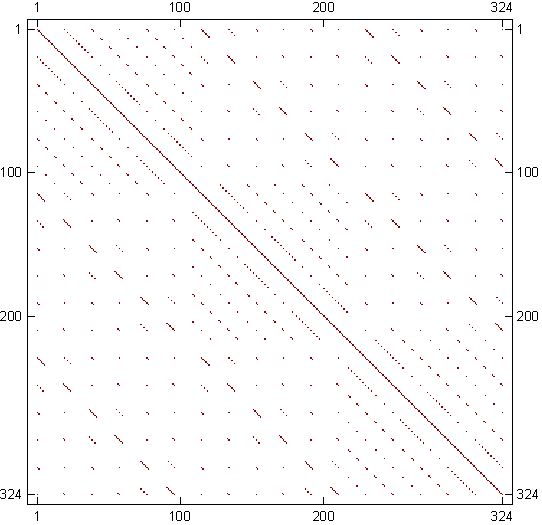
\includegraphics[scale=0.9]{images/matrixplot.pdf}
    \caption{Structure of scattering matrix associated with the $q\overline q \to q \overline q$ processes in the three-flavor scenario under the $U(2)^5$ flavor symmetry. The dimension of the matrix is $324=18^2$ as each $q$ or $\overline q$ contains $3\times 3\times 2$ degrees of freedom. To obtain its eigenvalues analytically, finite-field methods have been employed~\cite{Chestnov:2025svg}.}
    \label{fig:matrixplot}
\end{figure}

The same analysis has been carried out for all the remaining four-fermion operators. Since the
resulting set of flavor structures, bounds, and allowed regions is extensive, we collect it in
Appendix~\ref{app:SMEFT_flavorresults}.

\section{Phenomenological Applications\label{sec:SMEFT_pheno}}

To assess the phenomenological impact of the theoretical bounds discussed above, it is useful to examine their complementarity with both current and anticipated future experimental constraints.

We first analyze the unitarity bounds for purely bosonic operators. Figure~\ref{fig:histogram} shows the minimum energy scales $E_*$ at which the bounds in Table~\ref{tab:UniBounds} are violated, assuming Wilson coefficients are taken from the 95\% CL marginalized intervals of Ref.~\cite{Celada:2024mcf}, using linear (blue) and quadratic (orange) fits.
%
\begin{figure}[htbp]
    \centering
    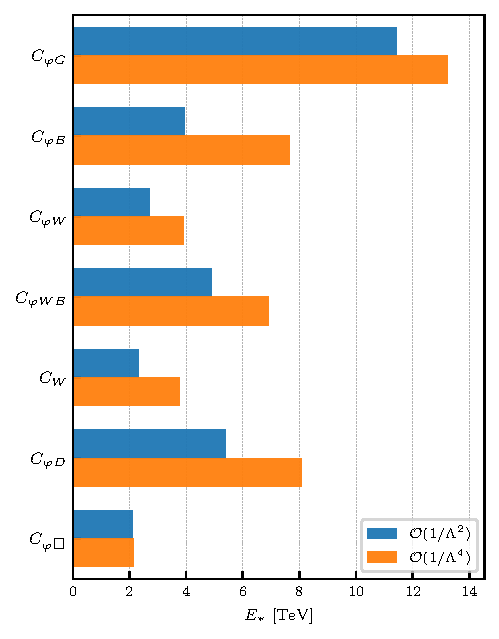
\includegraphics[scale=1.0]{images/histogram.pdf}
    \caption{Minimum energy scales $E_*$ at which the unitarity bounds in Table~\ref{tab:UniBounds} are violated for each purely bosonic Wilson coefficient in Ref.~\cite{Celada:2024mcf}, using the 95\% CL marginalized intervals from linear (blue) and quadratic (orange) fits.}
    \label{fig:histogram}
\end{figure}

Moreover, Figure~\ref{fig:3plotsa} presents both the unitarity bounds and the experimental constraints from LEP and (HL-)LHC diboson data on the Wilson coefficients of the operators $O_{\varphi q}^{(1)}$ and $O_{\varphi q}^{(3)}$.
\begin{figure}[htbp]
    \centering
    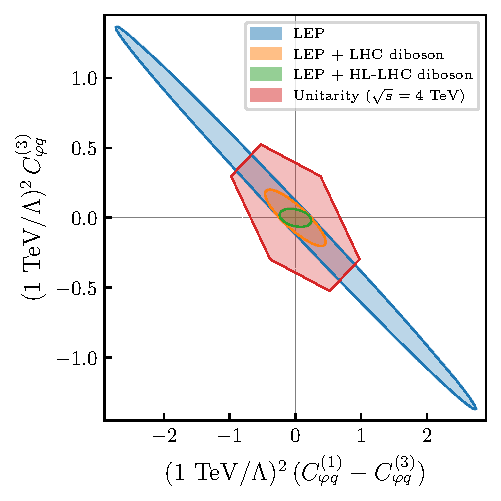
\includegraphics[scale=1]{images/dibosonv2.pdf}
    \caption{Experimental and unitarity constraints on the Wilson coefficients of the operators $O_{\varphi q}^{(1)} = \sum_{p=1,2}i(\varphi^\dagger \overset{\leftrightarrow}{D}{}_\mu \varphi)(\overline q_p \gamma^\mu q_p)$ and $O_{\varphi q}^{(3)} = \sum_{p=1,2}i(\varphi^\dagger \overset{\leftrightarrow}{D}{}_\mu^I \varphi)(\overline q_p \sigma^I \gamma^\mu q_p)$. Experimental limits correspond to $95\%$ CL marginalized intervals \cite{Celada:2024mcf}.}
    \label{fig:3plotsa}
\end{figure}
The experimental limits correspond to 95\% CL marginalized intervals obtained from a linear fit \cite{Celada:2024mcf}. As shown, the unitarity bounds --- scaling as $(\sqrt{s}/4~\mathrm{TeV})^2$ --- are significantly stronger than those from LEP alone, but remain weaker than the constraints derived from the combined LEP and (HL-)LHC data.

As a third example, we consider the global analysis of LHC Run II data in the top sector induced by the four-quark operators $O_{Qq}^{1,8}$ and $O_{Qq}^{3,8}$, where the experimental limits are obtained from a quadratic fit \cite{Brivio:2019ius}.
\begin{figure}[htbp]
    \centering
    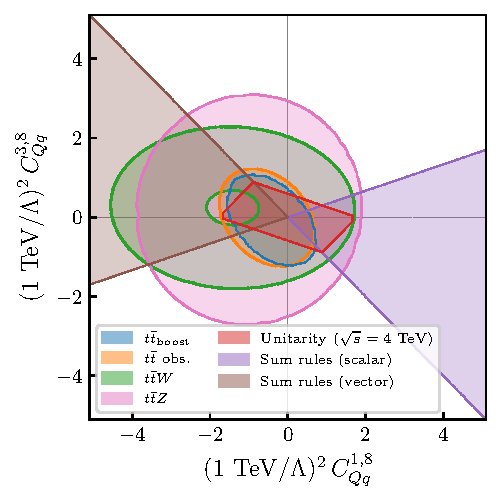
\includegraphics[scale=1]{images/top.pdf}
    \caption{Experimental and unitarity constraints on the Wilson coefficients of the 
    operators $O_{Qq}^{1,8} = \sum_{p=1,2}(\overline q_3 \gamma_\mu T^A q_3)(\overline q_p \gamma^\mu T^A q_p)$ and $O_{Qq}^{3,8} = \sum_{p=1,2}(\overline q_3 \gamma_\mu T^A \sigma^I q_3)(\overline q_p \gamma^\mu T^A \sigma^I q_p)$. 
    Experimental limits correspond to $68\%$ CL and are derived from a quadratic fit \cite{Brivio:2019ius}. Here, the sum rules select the region where $C_{Qq}^{1,8}-(1\pm 2)C_{Qq}^{3,8}$ are positive (negative) for scalar (vector) completions.}
    \label{fig:3plotsb}
\end{figure}
Most of the measurements involve final states with a top-quark pair, including kinematic distributions, the charge asymmetry, and associated top-pair production with a weak boson. As shown in Figure~\ref{fig:3plotsb}, the unitarity bounds are quite competitive with the LHC experimental limits. Interestingly, the inclusion of sum rules --- corresponding to an underlying scalar or vector tree-level mediator of the four-fermion interactions --- selects complementary regions of the parameter space, thereby providing insight into the nature of the underlying new-physics dynamics.

As a last example, we consider the comprehensive analysis of electroweak, flavor, and collider constraints on semileptonic 
four-fermion operators $[O_{\ell q}^{(1)}]_{3333}$ and $[O_{\ell q}^{(3)}]_{3333}$ in the $U(2)^5$ scenario of Ref.~\cite{Allwicher:2023shc}, where new physics predominantly couples to the third generation. Also in this case, as shown in Figure~\ref{fig:3plotsc}, the unitarity bounds and the sum-rule constraints are highly complementary and competitive with the experimental limits.
\begin{figure}[htbp]
    \centering
    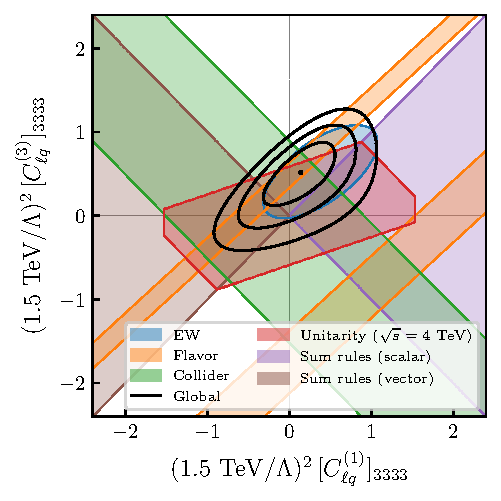
\includegraphics[scale=1]{images/flavor.pdf}
    \caption{Experimental and unitarity constraints on the Wilson coefficients of the 
    operators $[O_{\ell q}^{(1)}]_{3333} = (\overline \ell_3 \gamma^\mu \ell_3)(\overline q_3 \gamma_\mu q_3)$ and $[O_{\ell q}^{(3)}]_{3333} = (\overline \ell_3 \gamma^\mu \sigma^I \ell_3)(\overline q_3 \gamma_\mu \sigma^I q_3)$.
    Experimental limits correspond to $68\%$ CL \cite{Allwicher:2023shc}.}
    \label{fig:3plotsc}
\end{figure}
In particular, it is noteworthy that the $1\sigma$ region of the global fit lies outside the regions preferred by the sum rules. 
If the current experimental situation is confirmed and further strengthened, this would favor, for instance, an underlying $t$-channel UV completion.

These experimental contours are not recomputed by imposing an additional unitarity cut; the unitarity bounds should instead be interpreted as a theoretical consistency overlay.

As a final remark, the unitarity bounds constrain the
combination $\hat s|C|/\Lambda^2$, so that the
corresponding limits become increasingly stringent at
larger values of the partonic center-of-mass energy
$\sqrt{\hat s}$. Since perturbative unitarity determines
the range of validity of the EFT, the relevant scale
entering the bound is $\sqrt{\hat s}$, rather than the
collider center-of-mass energy itself. 

This is
particularly relevant for the HL-LHC: although it
operates at the same collider energy as the LHC, its
much larger integrated luminosity enables precision
measurements deeper into the high-energy tails of
differential distributions, thereby extending the range
of partonic scales over which the SMEFT description can
be meaningfully tested. Accordingly, while most collider
constraints discussed here probe partonic
center-of-mass energies of order
$\sqrt{\hat s}\sim 2$~TeV, we display the unitarity
bounds at $\sqrt{\hat s}=4$~TeV as a
representative benchmark for the multi-TeV regime
accessible in HL-LHC measurements. 

In realistic
analyses with a broad partonic energy spectrum, the
unitarity condition should instead be evaluated at the
value of $\sqrt{\hat s}$ relevant for each event or
kinematic bin, thereby defining the maximum hard scale
up to which the SMEFT description remains
perturbatively self-consistent.

\section{Conclusions\label{sec:SMEFT_conclusions}}

Non-renormalizable interactions induce scattering amplitudes that grow with energy, potentially
leading to violations of perturbative unitarity at high scales. A consistent interpretation of
experimental data, particularly at the High-Luminosity LHC and at future high-energy colliders,
therefore requires quantitative theoretical criteria to assess the range of validity of the SMEFT
description.

In this chapter we have performed a comprehensive reassessment of perturbative unitarity bounds on
all dimension-six SMEFT Wilson coefficients, significantly extending and sharpening the partial
results previously reported in the literature; see Table~\ref{tab:UniBounds}. The bound associated
with each Wilson coefficient was obtained by marginalizing over all the others, so that the numbers
quoted are conservative one-dimensional projections of the full coupled-channel unitarity region
rather than single-operator bounds; see Figures~\ref{fig:uni3} and
\ref{fig:1-flavor unitary+sum rules}. We performed a fully coupled-channel analysis, including all
allowed initial and final states across helicity, gauge, and flavor configurations, thereby deriving
stronger bounds than previously reported. In particular, we derived unitarity bounds for the complete
set of four-fermion operators as well as for operators involving gluon fields, which were not covered
in previous SMEFT studies~\cite{Corbett:2014ora,Corbett:2017qgl,Cao:2023qks}. The general $N\to M$
formalism of Chapter~\ref{ch:generalizedUB} was essential to treat all operator classes uniformly,
and in particular to constrain $O_\varphi$, which admits no $2\to2$ channel at all.

We then derived the spinning sum rules for four-fermion operators in the Warsaw basis and provided an operative procedure to translate them
into inequalities on the Wilson coefficients in flavor space. We also delimited their regime of
validity, identifying three distinct mechanisms through which they can fail and illustrated them with explicit UV completions.

Relaxing the single-flavor assumption, we presented the bounds on four-fermion operators under the
MFV and $U(2)^5$ flavor hypotheses, which reduce the $\mathcal O(1000)$ independent coefficients to
$\mathcal O(10)$ and make the multi-flavor analysis tractable.

As shown in Figures~\ref{fig:3plotsa}--\ref{fig:3plotsc}, these theoretical constraints are already
competitive with, and in some cases stronger than, the corresponding experimental bounds at energy
scales above a few TeV. This is particularly relevant for four-fermion operators under realistic
flavor assumptions motivated by the SM flavor puzzle, where the unitarity limits can be further
strengthened by imposing the sum rules. Interestingly, the sum rules select complementary regions of
the parameter space, thereby providing insight into the nature of the underlying new-physics
dynamics.

More broadly, the framework developed here establishes the first systematic, per\-tur\-ba\-ti\-vi\-ty-based
criterion that naturally incorporates operator correlations and can be directly implemented in
present and future global SMEFT analyses, collider phenomenology, and Monte Carlo event generation.
The results derived in this chapter strengthen the connection between theoretical and experimental
constraints in future searches for physics beyond the Standard Model.

\begin{subappendices}

\section{Conventions\label{app:SMEFT_conv}}
In Table~\ref{tab:WarsawBasis} we report the baryon-number-conserving dimension-six operators of the SMEFT in the Warsaw basis \cite{Grzadkowski:2010es}.
%
\begin{table}[tb]
\renewcommand{\arraystretch}{1.5}
    \centering
    \resizebox{\textwidth}{!}{
    \begin{tabular}{c | c|c | c|c| c|c| c|c| c}
    \toprule
    %\toprule
    \rowcolor{hdrcolor}
    \multicolumn{2}{c|}{{\boldmath$X^3$}} & \multicolumn{2}{c|}{{\boldmath$\varphi^6$}/{\boldmath$\varphi^4D^2$}} & \multicolumn{2}{c|}{{\boldmath$\psi^2\varphi^3$}} & \multicolumn{2}{c|}{{\boldmath$(\overline{L}L)(\overline{L}L)$}} & \multicolumn{2}{c}{{\boldmath$(\overline{L}R)(\overline{R}L)$}/{\boldmath$(\overline{L}R)(\overline{L}R)$}} \\
    \hline
    $O_G$ & $f^{ABC} G_\mu^{A\nu} G_\nu^{B\rho} G_\rho^{C\mu}$ & $O_\varphi$ & $(\varphi^\dagger \varphi)^3$ & $^\ddagger O_{e\varphi}$ & $(\varphi^\dagger \varphi)(\overline{\ell}_p e_r \varphi)$ & $O_{\ell\ell}$ & $(\overline{\ell}_p \gamma_\mu \ell_r)(\overline{\ell}_s \gamma^\mu \ell_t)$ & $^\ddagger O_{\ell edq}$ & $(\overline{\ell}_p^j e_r)(\overline{d}_s q_{tj})$ \\
    
    $O_{\widetilde{G}}$ & $f^{ABC} \widetilde{G}_\mu^{A\nu} G_\nu^{B\rho} G_\rho^{C\mu}$ & $O_{\varphi\Box}$ & $(\varphi^\dagger \varphi)\Box(\varphi^\dagger \varphi)$ & $^\ddagger O_{u\varphi}$ & $(\varphi^\dagger \varphi)(\overline{q}_p u_r \widetilde{\varphi})$ & $O_{qq}^{(1)}$ & $(\overline{q}_p \gamma_\mu q_r)(\overline{q}_s \gamma^\mu q_t)$ & $^\ddagger O_{quqd}^{(1)}$ & $(\overline{q}_p^j u_r)\epsilon_{jk}(\overline{q}_s^k d_t)$ \\
    
    $O_W$ & $\epsilon^{IJK} W_\mu^{I\nu} W_\nu^{J\rho} W_\rho^{K\mu}$ & $O_{\varphi D}$ & $(\varphi^\dagger D^\mu \varphi)^* (\varphi^\dagger D_\mu \varphi)$ & $^\ddagger O_{d\varphi}$ & $(\varphi^\dagger \varphi)(\overline{q}_p d_r \varphi)$ & $O_{qq}^{(3)}$ & $(\overline{q}_p \gamma_\mu \sigma^I q_r)(\overline{q}_s \gamma^\mu \sigma^I q_t)$ & $^\ddagger O_{quqd}^{(8)}$ & $(\overline{q}_p^j T^A u_r)\epsilon_{jk}(\overline{q}_s^k T^A d_t)$ \\
    
    $O_{\widetilde{W}}$ & $\epsilon^{IJK} \widetilde{W}_\mu^{I\nu} W_\nu^{J\rho} W_\rho^{K\mu}$ & & & & & $O_{\ell q}^{(1)}$ & $(\overline{\ell}_p \gamma_\mu \ell_r)(\overline{q}_s \gamma^\mu q_t)$ & $^\ddagger O_{\ell equ}^{(1)}$ & $(\overline{\ell}_p^j e_r)\epsilon_{jk}(\overline{q}_s^k u_t)$ \\
    
    & & & & & & $O_{\ell q}^{(3)}$ & $(\overline{\ell}_p \gamma_\mu \sigma^I \ell_r)(\overline{q}_s \gamma^\mu \sigma^I q_t)$ & $^\ddagger O_{\ell equ}^{(3)}$ & $(\overline{\ell}_p^j \sigma_{\mu\nu} e_r)\epsilon_{jk}(\overline{q}_s^k \sigma^{\mu\nu} u_t)$ \\
    
    \midrule
    %\midrule
    \rowcolor{hdrcolor}
    \multicolumn{2}{c|}{{\boldmath$X^2\varphi^2$}} & \multicolumn{2}{c|}{{\boldmath$\psi^2 X \varphi$}} & \multicolumn{2}{c|}{{\boldmath$\psi^2\varphi^2D$}} & \multicolumn{2}{c|}{{\boldmath$(\overline{R}R)(\overline{R}R)$}} & \multicolumn{2}{c}{{\boldmath$(\overline{L}L)(\overline{R}R)$}} \\
    \hline
    $O_{\varphi G}$ & $(\varphi^\dagger \varphi) G_{\mu\nu}^A G^{A\mu\nu}$ & $^\ddagger O_{eW}$ & $(\overline{\ell}_p \sigma^{\mu\nu} e_r)\sigma^I \varphi W_{\mu\nu}^I$ & $O_{\varphi\ell}^{(1)}$ & $(\varphi^\dagger i\overset{\leftrightarrow}{D}{}_\mu \varphi)(\overline{\ell}_p \gamma^\mu \ell_r)$ & $O_{ee}$ & $(\overline{e}_p \gamma_\mu e_r)(\overline{e}_s \gamma^\mu e_t)$ & $O_{\ell e}$ & $(\overline{\ell}_p \gamma_\mu \ell_r)(\overline{e}_s \gamma^\mu e_t)$ \\
    
    $O_{\varphi \widetilde{G}}$ & $(\varphi^\dagger \varphi) \widetilde{G}_{\mu\nu}^A G^{A\mu\nu}$ & $^\ddagger O_{eB}$ & $(\overline{\ell}_p \sigma^{\mu\nu} e_r)\varphi B_{\mu\nu}$ & $O_{\varphi\ell}^{(3)}$ & $(\varphi^\dagger i\overset{\leftrightarrow}{D}{}_\mu^I \varphi)(\overline{\ell}_p \sigma^I \gamma^\mu \ell_r)$ & $O_{uu}$ & $(\overline{u}_p \gamma_\mu u_r)(\overline{u}_s \gamma^\mu u_t)$ & $O_{\ell u}$ & $(\overline{\ell}_p \gamma_\mu \ell_r)(\overline{u}_s \gamma^\mu u_t)$ \\
    
    $O_{\varphi W}$ & $(\varphi^\dagger \varphi) W_{\mu\nu}^I W^{I\mu\nu}$ & $^\ddagger O_{uG}$ & $(\overline{q}_p \sigma^{\mu\nu} T^A u_r)\widetilde{\varphi} G_{\mu\nu}^A$ & $O_{\varphi e}$ & $(\varphi^\dagger i\overset{\leftrightarrow}{D}{}_\mu \varphi)(\overline{e}_p \gamma^\mu e_r)$ & $O_{dd}$ & $(\overline{d}_p \gamma_\mu d_r)(\overline{d}_s \gamma^\mu d_t)$ & $O_{\ell d}$ & $(\overline{\ell}_p \gamma_\mu \ell_r)(\overline{d}_s \gamma^\mu d_t)$ \\
    
    $O_{\varphi \widetilde{W}}$ & $(\varphi^\dagger \varphi) \widetilde{W}_{\mu\nu}^I W^{I\mu\nu}$ & $^\ddagger O_{uW}$ & $(\overline{q}_p \sigma^{\mu\nu} u_r)\sigma^I \widetilde{\varphi} W_{\mu\nu}^I$ & $O_{\varphi q}^{(1)}$ & $(\varphi^\dagger i\overset{\leftrightarrow}{D}{}_\mu \varphi)(\overline{q}_p \gamma^\mu q_r)$ & $O_{eu}$ & $(\overline{e}_p \gamma_\mu e_r)(\overline{u}_s \gamma^\mu u_t)$ & $O_{qe}$ & $(\overline{q}_p \gamma_\mu q_r)(\overline{e}_s \gamma^\mu e_t)$ \\
    
    $O_{\varphi B}$ & $(\varphi^\dagger \varphi) B_{\mu\nu} B^{\mu\nu}$ & $^\ddagger O_{uB}$ & $(\overline{q}_p \sigma^{\mu\nu} u_r)\widetilde{\varphi} B_{\mu\nu}$ & $O_{\varphi q}^{(3)}$ & $(\varphi^\dagger i\overset{\leftrightarrow}{D}{}_\mu^I \varphi)(\overline{q}_p \sigma^I \gamma^\mu q_r)$ & $O_{ed}$ & $(\overline{e}_p \gamma_\mu e_r)(\overline{d}_s \gamma^\mu d_t)$ & $O_{qu}^{(1)}$ & $(\overline{q}_p \gamma_\mu q_r)(\overline{u}_s \gamma^\mu u_t)$ \\
    
    $O_{\varphi \widetilde{B}}$ & $(\varphi^\dagger \varphi) \widetilde{B}_{\mu\nu} B^{\mu\nu}$ & $^\ddagger O_{dG}$ & $(\overline{q}_p \sigma^{\mu\nu} T^A d_r)\varphi G_{\mu\nu}^A$ & $O_{\varphi u}$ & $(\varphi^\dagger i\overset{\leftrightarrow}{D}{}_\mu \varphi)(\overline{u}_p \gamma^\mu u_r)$ & $O_{ud}^{(1)}$ & $(\overline{u}_p \gamma_\mu u_r)(\overline{d}_s \gamma^\mu d_t)$ & $O_{qu}^{(8)}$ & $(\overline{q}_p \gamma_\mu T^A q_r)(\overline{u}_s \gamma^\mu T^A u_t)$ \\
    
    $O_{\varphi WB}$ & $(\varphi^\dagger \sigma^I \varphi) W_{\mu\nu}^I B^{\mu\nu}$ & $^\ddagger O_{dW}$ & $(\overline{q}_p \sigma^{\mu\nu} d_r)\sigma^I \varphi W_{\mu\nu}^I$ & $O_{\varphi d}$ & $(\varphi^\dagger i\overset{\leftrightarrow}{D}{}_\mu \varphi)(\overline{d}_p \gamma^\mu d_r)$ & $O_{ud}^{(8)}$ & $(\overline{u}_p \gamma_\mu T^A u_r)(\overline{d}_s \gamma^\mu T^A d_t)$ & $O_{qd}^{(1)}$ & $(\overline{q}_p \gamma_\mu q_r)(\overline{d}_s \gamma^\mu d_t)$ \\
    
    $O_{\varphi \widetilde{W}B}$ & $(\varphi^\dagger \sigma^I \varphi) \widetilde{W}_{\mu\nu}^I B^{\mu\nu}$ & $^\ddagger O_{dB}$ & $(\overline{q}_p \sigma^{\mu\nu} d_r)\varphi B_{\mu\nu}$ & $^\ddagger O_{\varphi ud}$ & $(\widetilde{\varphi}^\dagger i D_\mu \varphi)(\overline{u}_p \gamma^\mu d_r)$ & & & $O_{qd}^{(8)}$ & $(\overline{q}_p \gamma_\mu T^A q_r)(\overline{d}_s \gamma^\mu T^A d_t)$ \\
    \bottomrule
    %\bottomrule
    \end{tabular}
    }
    \caption{Dimension-six operators of the SMEFT in the Warsaw basis~\cite{Grzadkowski:2010es} that conserve baryon number. Non-Hermitian operators are denoted with $^\ddagger O$ and the corresponding Hermitian conjugates must be included in the Lagrangian.}
    \label{tab:WarsawBasis}
\end{table}

The relevant conventions are as follows: $\widetilde \varphi^j = \epsilon^{jk} (\varphi^k)^*$ (with $\epsilon^{12}=1$), $\varphi^\dagger \overset{\leftrightarrow}{D}{}_\mu \varphi = \varphi^\dagger D_\mu \varphi - (D_\mu \varphi)^\dagger \varphi$ and $\varphi^\dagger \overset{\leftrightarrow}{D}{}_\mu^I \varphi = \varphi^\dagger \sigma^I D_\mu \varphi - (D_\mu \varphi)^\dagger \sigma^I \varphi$, dual field-strength tensors are defined as $\widetilde X_{\mu\nu} = \frac{1}{2}\epsilon_{\mu\nu\rho\sigma}X^{\rho\sigma}$ (with $X=B,W^I,G^A$ and $\epsilon^{0123} = 1$), $\lambda^A_{\alpha\beta}$ are the Gell-Mann matrices and $\sigma^I_{jk}$ are the Pauli matrices, $T_{\alpha\beta}^A = \frac{1}{2}\lambda^A_{\alpha\beta}$ are the $SU(3)$ generators, and $\sigma_{\mu\nu} = \frac{i}{2}[\gamma_\mu,\gamma_\nu]$.
The Minkowski metric, whose signature is relevant for the spinning sum rules, is $g_{\mu\nu} = \operatorname{diag}(+1,-1,-1,-1)$.

\section{Matching of Ultraviolet Completions\label{app:SMEFT_UV}}

To illustrate both the diagnostic power and the limitations of the spinning sum
rules discussed in Section~\ref{sec:SMEFT_sumrules}, we match a
representative set of single-field, tree-level UV completions \cite{deBlas:2017xtg}
onto the third-generation semileptonic operators $[O_{\ell q}^{(1)}]_{3333}$ and
$[O_{\ell q}^{(3)}]_{3333}$, whose unitarity and sum-rule constraints are shown in
Figure~\ref{fig:3plotsc}. The results are collected in Table~\ref{tab:models}.
%
\begin{table}[tb]
\renewcommand{\arraystretch}{1}
    \centering
    \resizebox{\textwidth}{!}{
    \begin{tabular}{ccccccc}
    %\toprule
    \toprule
    \rowcolor{hdrcolor}
    \textbf{Field}  & \textbf{Spin} & \textbf{Channel} & \boldmath$[C_{\ell q}^{(1)}]_{3333}/\Lambda^2$ & \boldmath$[C_{\ell q}^{(3)}]_{3333}/\Lambda^2$ & \textbf{Unitarity Bound} & \textbf{Plot} \\
    \midrule
    % $\omega_1$ & $(3,1)_{-\displaystyle\frac{1}{3}}$ & $0$ & $s$ & $\displaystyle\frac{|[y^{q\ell}_{\omega_1}]_{33}|^2}{4M^2_{\omega_1}}$ & $\displaystyle\frac{-|[y^{q\ell}_{\omega_1}]_{33}|^2}{4M^2_{\omega_1}}$ & $\displaystyle\frac{|[y^{q\ell}_{\omega_1}]_{33}|^2 s}{4\pi M^2_{\omega_1}}\leq 1$ & \makecell[c]{\includegraphics[scale = 0.5]{images/omega1.pdf}} \\
    % $\zeta$ & $(3,3)_{-\displaystyle\frac{1}{3}}$ & $0$ & $s$ & $3|[y^{q\ell}_{\zeta}]_{33}|^2/(4M^2_{\zeta})$ & $|[y^{q\ell}_{\zeta}]_{33}|^2/(4M^2_{\zeta})$ & $|[y^{q\ell}_{\zeta}]_{33}|^2\,s\leq 4\pi M^2_{\zeta}$ & \makecell[c]{\includegraphics[scale = 0.5]{images/zeta.pdf}} \\
    % $\mathcal{U}_2$ & $(3,1)_{\displaystyle\frac{2}{3}}$ & $1$ & $s$ & $-|[g_{\mathcal U_2}^{\ell q}]_{33}|^2/(2M^2_{\mathcal U_2})$ & $-|[g_{\mathcal U_2}^{\ell q}]_{33}|^2/(2M^2_{\mathcal U_2})$ & $|[g_{\mathcal U_2}^{\ell q}]_{33}|^2\,s\leq 4\pi M^2_{\mathcal U_2}$ & \makecell[c]{\includegraphics[scale = 0.5]{images/U2.pdf}} \\
    % $\mathcal{X}$ & $(3,3)_{\displaystyle\frac{2}{3}}$ & $1$ & $s$ & $-3|[g_{\mathcal X}]_{33}|^2/(8M^2_{\mathcal X})$ & $|[g_{\mathcal X}]_{33}|^2/(8M^2_{\mathcal X})$ & $|[g_{\mathcal X}]_{33}|^2\,s\leq \tfrac{16}{3}\pi M^2_{\mathcal X}$ & \makecell[c]{\includegraphics[scale = 0.5]{images/X.pdf}} \\
    % $\mathcal{B}$ & $(1,1)_{0}$ & $1$ & $t$ & $-[g_{\mathcal B}^\ell]_{33}[g_{\mathcal B}^q]_{33}/M^2_{\mathcal B}$ & $0$ & $|[g_{\mathcal B}^\ell]_{33}[g_{\mathcal B}^q]_{33}|\,s\leq 2\sqrt{3}\,\pi M^2_{\mathcal B}$ & \makecell[c]{\includegraphics[scale = 0.5]{images/B.pdf}} \\
    % $\mathcal{W}$ & $(1,3)_{0}$ & $1$ & $t$ & $0$ & $-[g_{\mathcal W}^\ell]_{33}[g_{\mathcal W}^q]_{33}/(4M^2_{\mathcal W})$ & $|[g_{\mathcal W}^\ell]_{33}[g_{\mathcal W}^q]_{33}|\,s\leq \tfrac{16}{3}\pi M^2_{\mathcal W}$ & \makecell[c]{\includegraphics[scale = 0.5]{images/W.pdf}} \\
    % \bottomrule
    $\omega_1\sim(3,1)_{-\frac{1}{3}}$ & $0$ & $s$ & $\displaystyle\frac{|[y^{q\ell}_{\omega_1}]_{33}|^2}{4M^2_{\omega_1}}$ & $\displaystyle\frac{-|[y^{q\ell}_{\omega_1}]_{33}|^2}{4M^2_{\omega_1}}$ & $\displaystyle\frac{|[y^{q\ell}_{\omega_1}]_{33}|^2 s}{4\pi M^2_{\omega_1}}\leq 1$ & \makecell[c]{\includegraphics[scale = 0.8,page=6]{images/UVfield.pdf}} \\
$\zeta\sim(3,3)_{-\frac{1}{3}}$ & $0$ & $s$ & $\displaystyle\frac{3|[y^{q\ell}_{\zeta}]_{33}|^2}{4M^2_{\zeta}}$ & $\displaystyle\frac{|[y^{q\ell}_{\zeta}]_{33}|^2}{4M^2_{\zeta}}$ & $\displaystyle\frac{|[y^{q\ell}_{\zeta}]_{33}|^2s}{4\pi M^2_{\zeta}}\leq 1$ & \makecell[c]{\includegraphics[scale = 0.8,page=5]{images/UVfield.pdf}} \\
$\mathcal{U}_2\sim(3,1)_{\frac{2}{3}}$ & $1$ & $s$ & $\displaystyle\frac{-|[g_{\mathcal U_2}^{\ell q}]_{33}|^2}{2M^2_{\mathcal U_2}}$ & $\displaystyle\frac{-|[g_{\mathcal U_2}^{\ell q}]_{33}|^2}{2M^2_{\mathcal U_2}}$ & $\displaystyle\frac{|[g_{\mathcal U_2}^{\ell q}]_{33}|^2s}{4\pi M^2_{\mathcal U_2}}\leq 1$ & \makecell[c]{\includegraphics[scale = 0.8,page=4]{images/UVfield.pdf}} \\
$\mathcal{X}\sim(3,3)_{\frac{2}{3}}$ & $1$ & $s$ & $\displaystyle\frac{-3|[g_{\mathcal X}]_{33}|^2}{8M^2_{\mathcal X}}$ & $\displaystyle\frac{|[g_{\mathcal X}]_{33}|^2}{8M^2_{\mathcal X}}$ & $\displaystyle\frac{3|[g_{\mathcal X}]_{33}|^2s}{16\pi M^2_{\mathcal X}}\leq 1$ & \makecell[c]{\includegraphics[scale = 0.8,page=3]{images/UVfield.pdf}} \\
$\mathcal{B}\sim(1,1)_{0}$ & $1$ & $t$ & $\displaystyle\frac{-[g_{\mathcal B}^\ell]_{33}[g_{\mathcal B}^q]_{33}}{M^2_{\mathcal B}}$ & $0$ & $\displaystyle\frac{|[g_{\mathcal B}^\ell]_{33}[g_{\mathcal B}^q]_{33}|s}{2\sqrt{3}\pi M^2_{\mathcal B}}\leq 1$ & \makecell[c]{\includegraphics[scale = 0.8,page=2]{images/UVfield.pdf}} \\
$\mathcal{W}\sim(1,3)_{0}$ & $1$ & $t$ & $0$ & $\displaystyle\frac{-[g_{\mathcal W}^\ell]_{33}[g_{\mathcal W}^q]_{33}}{4M^2_{\mathcal W}}$ & $\displaystyle\frac{3|[g_{\mathcal W}^\ell]_{33}[g_{\mathcal W}^q]_{33}|s}{16\pi M^2_{\mathcal W}}\leq 1$ & \makecell[c]{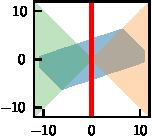
\includegraphics[scale = 0.8,page=1]{images/UVfield.pdf}} \\
\bottomrule
    \end{tabular}
    }
    \caption{Tree-level matching of single-field UV completions \cite{deBlas:2017xtg}
    onto $[O_{\ell q}^{(1)}]_{3333}$ and $[O_{\ell q}^{(3)}]_{3333}$. The penultimate
    column reports the associated perturbative unitarity bound, obtained as the most
    stringent of the constraints for $[C_{\ell q}^{(1)}]_{3333}$ and $[C_{\ell q}^{(3)}]_{3333}$ evaluated on the
    matched Wilson coefficients. The last column contains the plots in the plane $(s[C_{\ell q}^{(1)}]_{3333}/\Lambda^2, s[C_{\ell q}^{(3)}]_{3333}/\Lambda^2)$, where the blue, orange, and green regions correspond to those consistent with unitarity bounds and spin-$0$ and spin-$1$ sum-rule constraints, respectively, while the red lines indicate where each model lies: the scalar and vector leptoquarks are correctly classified by
    their spin, whereas the $t$-channel vectors evade the classification.}
    \label{tab:models}
\end{table}

The two scalar leptoquarks ($\omega_1$, $\zeta$) and the two vector leptoquarks
($\mathcal{U}_2$, $\mathcal{X}$) generate these operators through $s$-channel
exchange in the elastic $\ell q \to \ell q$ amplitude, and therefore enter the
dispersion relation of Eq.~\eqref{eq: sum rules master equation} with their physical
spin. 
Explicitly, the relevant combinations of Table~\ref{tab:sum_rules},
$[C_{\ell q}^{(1)}]_{3333} \pm [C_{\ell q}^{(3)}]_{3333}$, are both non-negative for
$\omega_1$ and $\zeta$, and both non-positive for $\mathcal{U}_2$ and $\mathcal{X}$,
so that the scalar (vector) leptoquarks are correctly placed in the scalar-
(vector-) dominated region of Figure~\ref{fig:3plotsc}.

By contrast, the color-singlet vectors $\mathcal{B} \sim (1,1)_0$ and
$\mathcal{W} \sim (1,3)_0$ couple separately to the lepton and quark currents and are exchanged in the $t$-channel. The boundary terms then no longer vanish, modifying Eq.~\eqref{eq: sum rules master equation}, and the sum-rule
classification fails: $\mathcal{W}$ yields combinations of opposite sign and thus
lies outside both the scalar- and vector-dominated regions, while $\mathcal{B}$ can
fall in the region associated with the opposite (scalar) spin, depending on the sign
of $[g_{\mathcal B}^\ell]_{33}[g_{\mathcal B}^q]_{33}$. These cases provide explicit
examples of the statement made in the main text that vector $t$-channel completions
can violate the spinning sum-rule constraints, whereas all tree-level scalar
completions satisfy them.

\section{Mathematical Tools\label{app:SMEFT_math}}

\subsection{Logical Expression}\label{sec:appendix, logical expression}

In this appendix we prove the statement used in Section~\ref{sec:SMEFT_sumrules}. The function
\begin{equation}
    f(x) = a + bx - \sqrt{c^2 + dx + ex^2}\,,
\end{equation}
assumed real on $[0,1]$ and with $a,b,c,d,e\in\mathbb{R}$, satisfies $f(x) \ge 0$ for every
$x \in [0,1]$ if and only if
\begin{align}
    \Delta(a,b,c,d,e) &= 
    a \ge 0 
    \ \land \
    a+b \ge 0
    \ \land \ 
    a^2 - c^2 \ge 0
    \ \land \ 
    (a+b)^2 - c^2 -d-e \ge 0 \nonumber
    \\& \quad
    \land \
    [e - b^2 \ge 0 \ \lor\  (2ab-d)(2ab-d+2b^2-2e) \ge 0 
    \nonumber \\& \quad
    \lor \ 4(b^2-e)(a^2-c^2)-(2ab-d)^2 \ge 0]
\end{align}
holds, which is the condition quoted in Eq.~\eqref{eq:Delta} of the main text.

Since $g(x)=c^2 + dx + ex^2 \ge 0$ on $[0,1]$ by assumption, $f(x) \ge 0$ on $[0,1]$ is equivalent to $\ell(x) = a + bx \ge 0$ and $h(x) = \ell(x)^2 -g(x) \ge 0$ on $[0,1]$. The latter reads $h(x) = \alpha x^2 + \beta x + \gamma$, with $\alpha = b^2-e$, $\beta = 2ab-d$, and $\gamma=a^2-c^2$.
Thus, it is sufficient to prove that $p(x) = \alpha x^2+\beta x + \gamma \ge 0$ on $[0,1]$ if and only if
    \begin{equation}\label{eq:lemma}
        \gamma\ge0 \ \land \ \alpha+\beta+\gamma\ge0 \ \land \
    [\alpha\le0 \ \lor \ \beta(\beta+2\alpha)\ge0 \ \lor \ 4\alpha\gamma-\beta^2\ge0 ] \,.
    \end{equation}
Indeed, Eq.~\eqref{eq:Delta} is exactly Eq.~\eqref{eq:lemma} applied to $\ell$ and $h$.
The first two conditions in Eq.~\eqref{eq:lemma} are $p(0)\ge 0$ and $p(1)\ge 0$, thus they are necessary; assume them in what follows. If $\alpha \le 0$, then $p$ is concave and has its minimum on $[0,1]$ at an endpoint, so $p\ge 0$; instead, if $\alpha >0$, the vertex is at $x_\ast = -\beta/(2\alpha)$, and
\begin{equation}
    x_\ast\le0 \iff \beta\ge0 \,, \qquad x_\ast\ge1 \iff \beta+2\alpha\le0 \,,
\end{equation}
so $x_\ast \notin (0,1)$ if and only if $\beta(\beta+2\alpha)\ge 0$, in which case the minimum is again at an endpoint and $p\ge 0$. Otherwise, $x_\ast \in (0,1)$ and $\min_{[0,1]} p = p(x_\ast) = (4\alpha\gamma-\beta^2)/(4\alpha)$, which has the same sign as $4\alpha\gamma-\beta^2$. The last condition is then both necessary and sufficient. 

\subsection{Eigenvalues of Jordan--Wielandt Matrices}

Given the Hermitian Jordan--Wielandt matrix
\begin{equation}
    M=\begin{pmatrix}
        \mathbb{O}_{m\times m} & A \\ A^\dagger & \mathbb{O}_{n\times n}
    \end{pmatrix}
\end{equation}
of size $m+n$,
with $A\in \mathbb{C}^{m \times n}$,
we have that its characteristic polynomial --- with the convention $p_X(x) = \det(x\mathbb{1}-X)$ --- is
\begin{equation}
    p_M(x)=x^{n-m}\,p_{AA^\dagger}(x^2) = x^{m-n}\,p_{A^\dagger A}(x^2) \,,
\end{equation}
which means that the eigenvalues of $M$ can be computed as the positive and negative square roots of the eigenvalues of $AA^\dagger$ if $m\le n$ (of $A^\dagger A$ if $m > n$), together with additional $\abs{n-m}$ vanishing eigenvalues. 
%

To prove this, consider a generic block matrix that takes the form
\begin{equation}
    \begin{pmatrix}
        P & Q \\ R & S
    \end{pmatrix}\,.
\end{equation}
If $S$ is invertible, then
\begin{equation}
    \begin{pmatrix}
        P & Q \\ R & S
    \end{pmatrix}
    \begin{pmatrix} \mathbb{1} & \mathbb{O} \\ -S^{-1}R & \mathbb{1} 
    \end{pmatrix}
    =
    \begin{pmatrix} P-QS^{-1}R & Q \\ \mathbb{O} & S 
    \end{pmatrix}\,,
\end{equation}
which implies that 
\begin{equation}
    \det\begin{pmatrix} P & Q \\ R & S \end{pmatrix}=\det(P-QS^{-1}R) \det S \,.
\end{equation}
By applying this to the matrix $x\mathbb{1}_{(m+n)\times(m+n)}-M$, we find the result above.

\section{Complete Results for Flavorful Four-Fermion Operators\label{app:SMEFT_flavorresults}}

In this appendix we collect the marginalized partial-wave unitarity bounds and the corresponding
allowed regions for all the four-fermion operators under the MFV and $U(2)^5$ flavor hypotheses,
obtained with the procedure described in Section~\ref{sec:SMEFT_multiflavor}. For each operator we
report the independent flavor structures and the bound on each independent coefficient.
Table~\ref{tab:summary} serves as an index to the tables and figures that follow. The case of
$O_{\ell q}^{(1,3)}$, used as an illustration in the main text, is reported in
Table~\ref{tab:Olq_UB} and in Figures~\ref{fig:Olq_mfv} and \ref{fig:Olq_u2}.

\begin{table}[tbp]
\renewcommand{\arraystretch}{1.2}
    \centering
    \begin{tabular}{cccc}
    \toprule
    \rowcolor{hdrcolor} \textbf{Operator class}     & \textbf{Operator(s)} & \textbf{Table} & \textbf{Figure(s)}  \\
    \midrule
    \multirow{3}{*}{\boldmath$(\overline LL)(\overline LL)$}     & $O_{\ell \ell}$ &\ref{tab:Oll_UB} & \ref{fig:Oll_mfv} (MFV), \ref{fig:Oll_u2} ($\mathrm{U}(2)^5$)  \\
    & $O_{qq}^{(1,3)}$ &\ref{tab:Oqq_UB}&\ref{fig:Oqq_mfv} (MFV), \ref{fig:Oqq_u2} ($\mathrm{U}(2)^5$) \\
    & $O_{\ell q}^{(1,3)}$ &\ref{tab:Olq_UB}& \ref{fig:Olq_mfv} (MFV), \ref{fig:Olq_u2} ($\mathrm{U}(2)^5$) \\
    \midrule
    \multirow{6}{*}{\boldmath$(\overline RR)(\overline RR)$} & $O_{ee}$ & \ref{tab:Oee_UB} & \ref{fig:Oee_u2} ($\mathrm{U}(2)^5$)  \\
    & $O_{uu}$ &\ref{tab:Ouu_UB}&\ref{fig:Ouu_mfv} (MFV), \ref{fig:Ouu_u2} ($\mathrm{U}(2)^5$) \\
    & $O_{dd}$ &\ref{tab:Odd_UB}& \ref{fig:Odd_mfv} (MFV), \ref{fig:Ouu_u2} ($\mathrm{U}(2)^5$) \\
    & $O_{eu}$ &\ref{tab:Oeu_UB}& \ref{fig:Oeu_mfv} (MFV), \ref{fig:Oeu_u2} ($\mathrm{U}(2)^5$)  \\
    & $O_{ed}$ &\ref{tab:Oed_UB}&  \ref{fig:Oeu_u2} ($\mathrm{U}(2)^5$) \\
    & $O_{ud}^{(1,8)}$ &\ref{tab:Oud_UB}& \ref{fig:Oud_mfv} (MFV), \ref{fig:Oud_u2} ($\mathrm{U}(2)^5$) \\
    \midrule
    \multirow{6}{*}{\boldmath$(\overline LL)(\overline RR)$} & $O_{\ell e}$ &\ref{tab:Ole_UB} &  \ref{fig:Ole_u2} ($\mathrm{U}(2)^5$)  \\
    & $O_{\ell u}$ &\ref{tab:Olu_UB}& \ref{fig:Olu_mfv} (MFV), \ref{fig:Olu_u2} ($\mathrm{U}(2)^5$) \\
    & $O_{\ell d}$ &\ref{tab:Old_UB}&  \ref{fig:Olu_u2} ($\mathrm{U}(2)^5$) \\
    & $O_{qe}$ &\ref{tab:Oqe_UB}& \ref{fig:Oqe_mfv} (MFV), \ref{fig:Oqe_u2} ($\mathrm{U}(2)^5$) \\
    & $O_{qu}^{(1,8)}$ &\ref{tab:Oqu_UB}& \ref{fig:Oqu_mfv} (MFV), \ref{fig:Oqu_u2} ($\mathrm{U}(2)^5$) \\
    & $O_{qd}^{(1,8)}$ &\ref{tab:Oqd_UB}& \ref{fig:Oqd_mfv} (MFV), \ref{fig:Oqu_u2} ($\mathrm{U}(2)^5$) \\
    \bottomrule
    \end{tabular}
    \caption{Hyperlinks to tables of marginalized partial-wave unitarity bounds and figures of the corresponding constraint regions in the MFV and $\mathrm{U}(2)^5$ flavor symmetry scenarios.}
    \label{tab:summary}
\end{table}

\input{tables/tables_flavor_rest}



\begin{figure}[p]
    \centering
    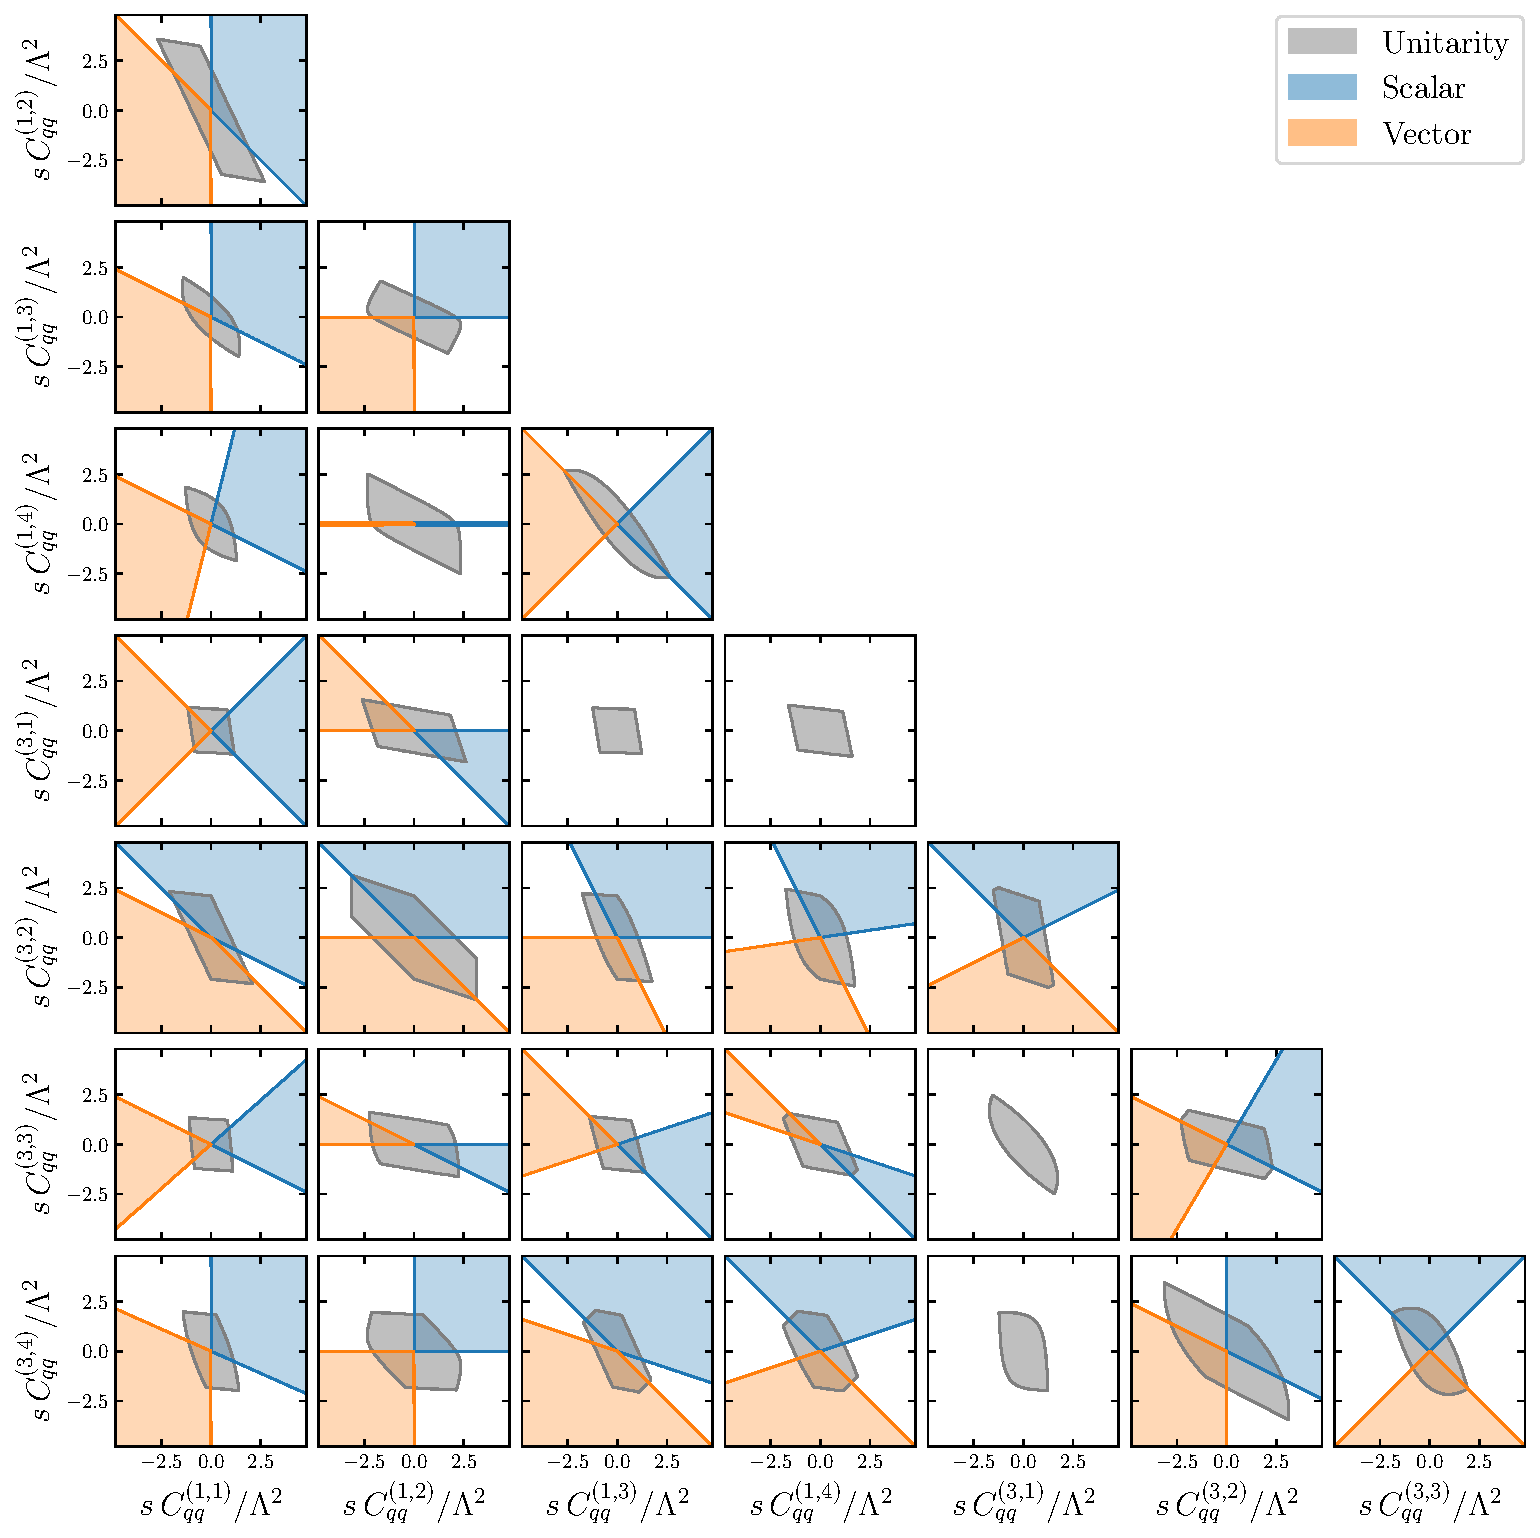
\includegraphics[width=1\linewidth]{images/flavor/Oqq_mfv.pdf}
    \caption{Partial-wave unitarity bounds and sum-rule constraints (under scalar and vector dominance) for the operators $O_{qq}^{(1,3)}$ under MFV, where $[C_{qq}^{(i)}]_{prst} =
            C_{qq}^{(i,1)}\delta_{pr}\delta_{st}
            + C_{qq}^{(i,2)}\delta_{pt}\delta_{sr}
            + C_{qq}^{(i,3)}((Y_u Y_u^\dagger)_{st}\delta_{pr} + (Y_u Y_u^\dagger)_{pr}\delta_{st}) + C_{qq}^{(i,4)}((Y_u Y_u^\dagger)_{sr}\delta_{pt} + (Y_u Y_u^\dagger)_{pt}\delta_{sr})$, $i=1,3$. The regions shown are two-dimensional slices of the full allowed region, obtained by setting to zero all the independent coefficients other than the two displayed.}
    \label{fig:Oqq_mfv}
\end{figure}

\begin{figure}[p]
    \centering
    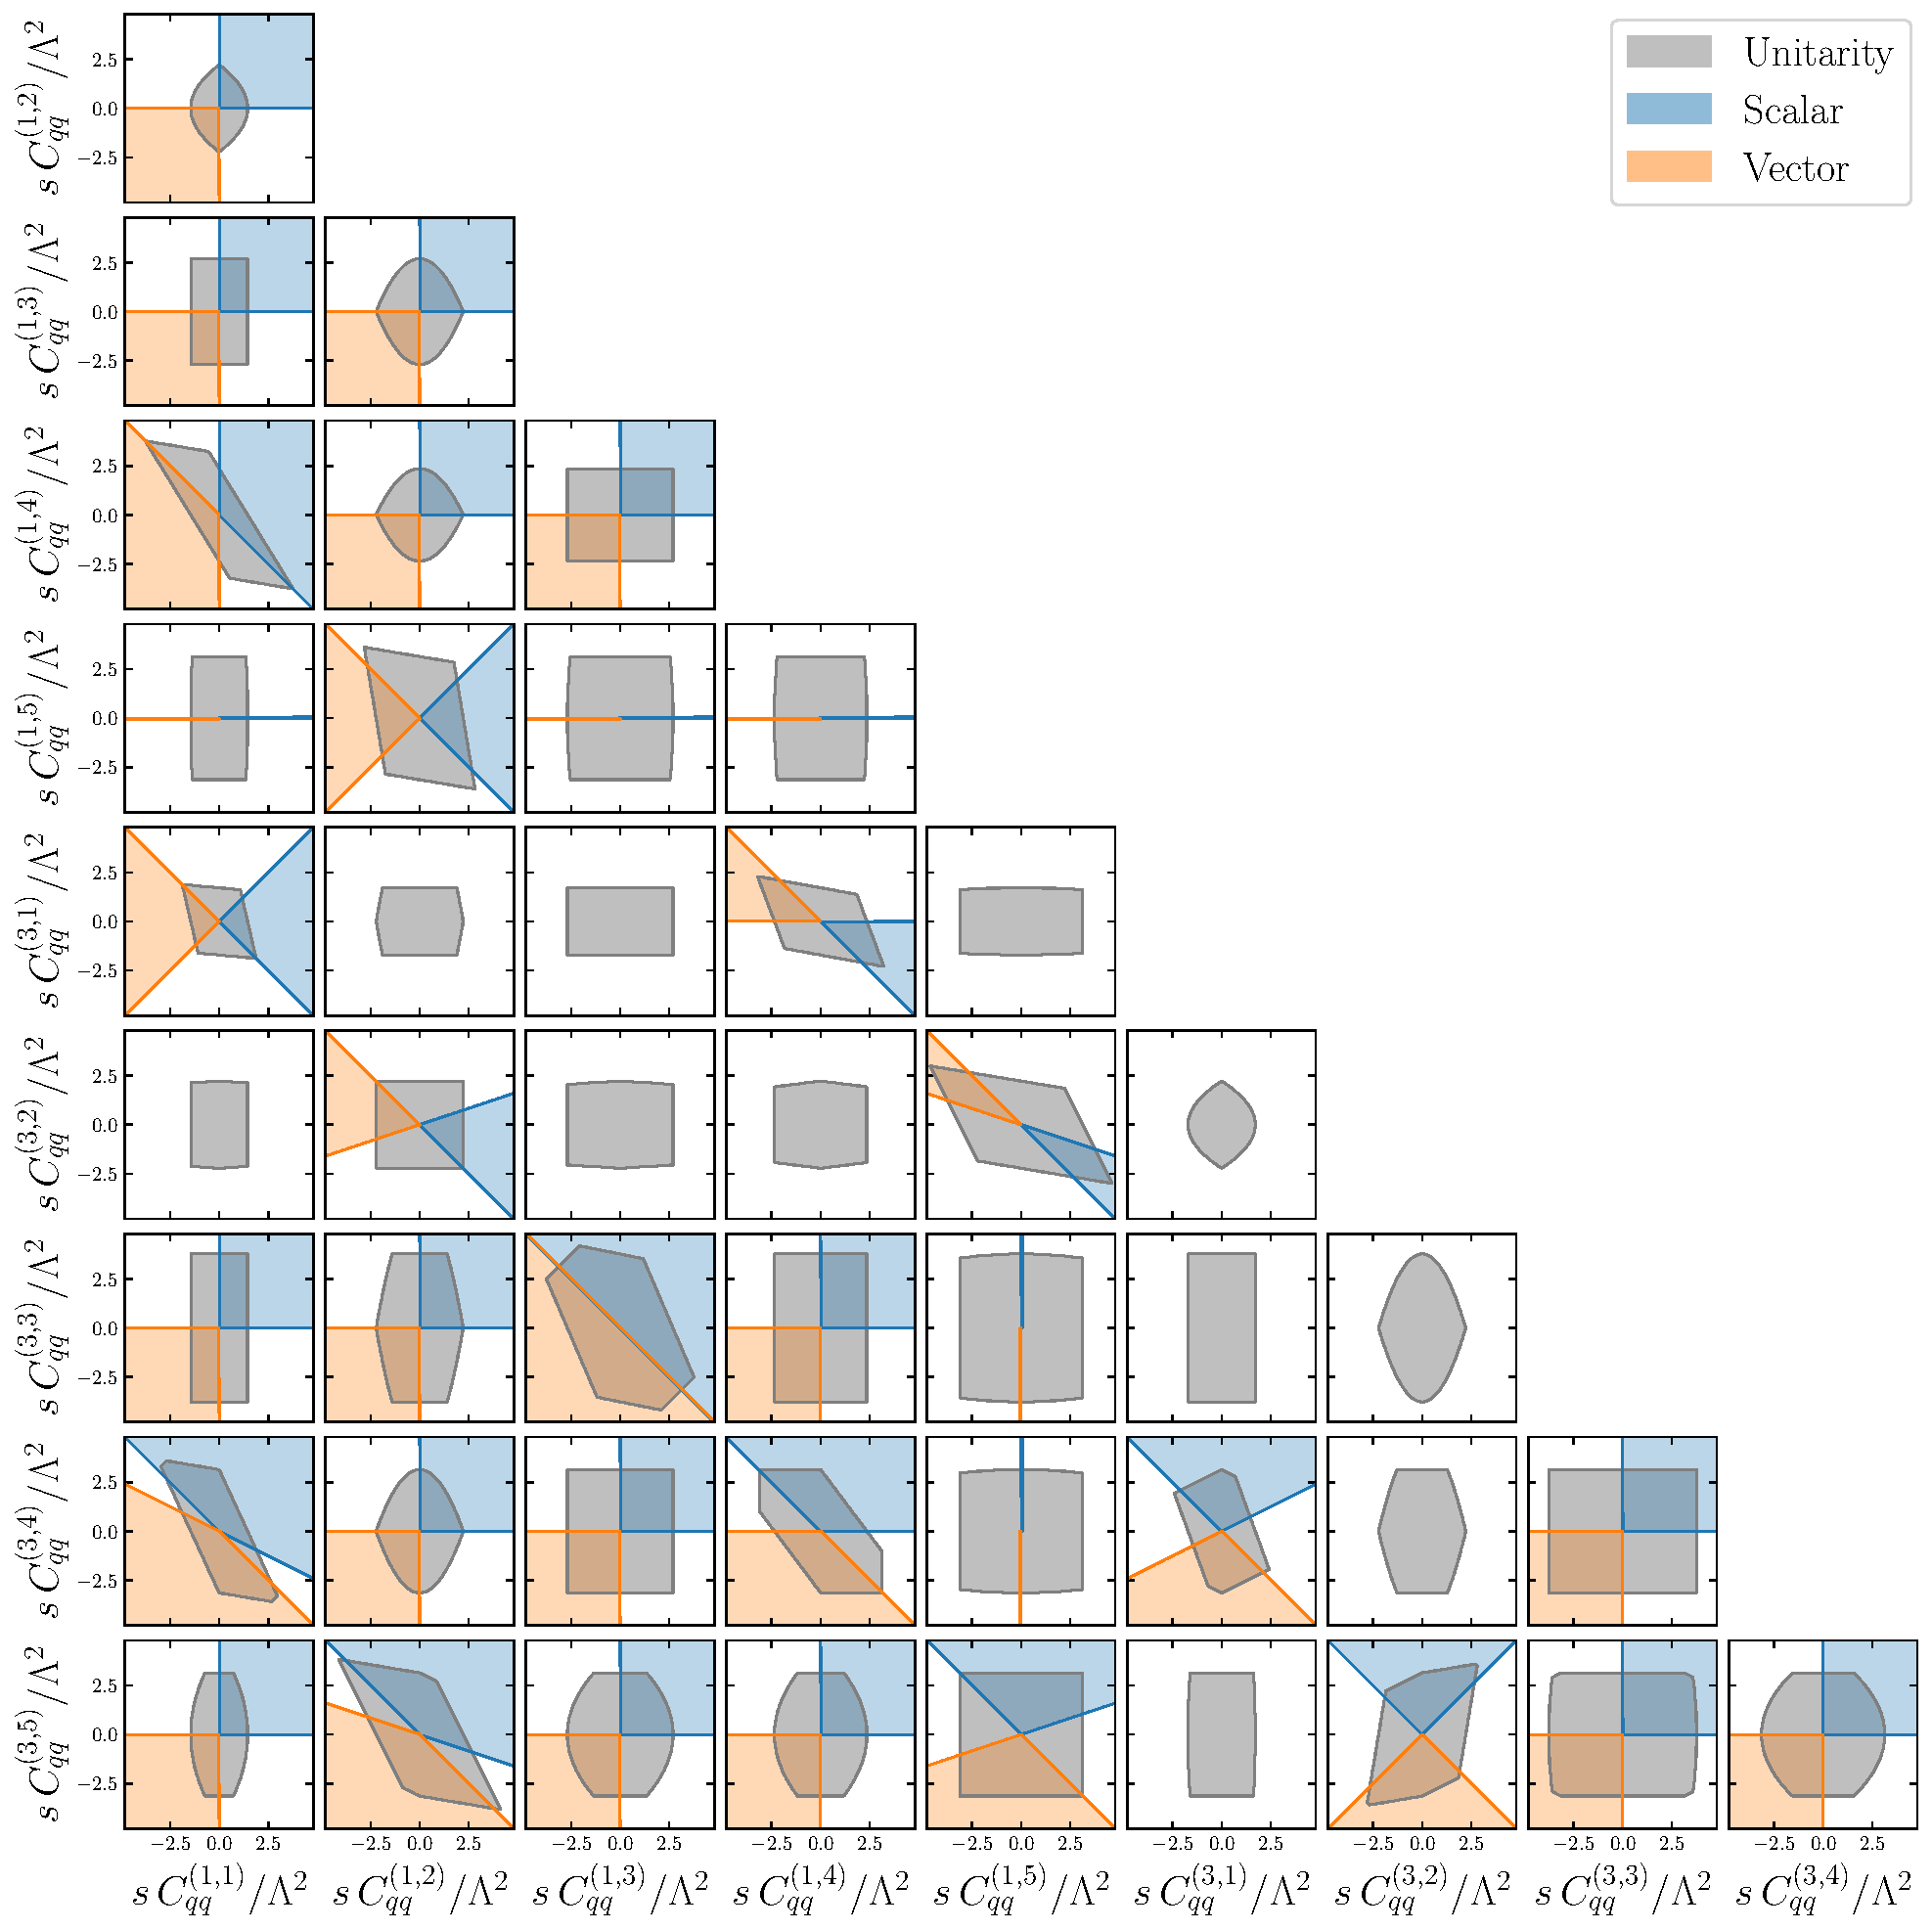
\includegraphics[width=1\linewidth]{images/flavor/Oqq_u2.pdf}
    \caption{Partial-wave unitarity bounds and sum-rule constraints (under scalar and vector dominance) for the operators $O_{qq}^{(i)}$ under $U(2)^5$ flavor symmetry, where $[C_{qq}^{(i)}]_{prst} =
            C_{qq}^{(i,1)}\Pij{p}{r}{a}\Pij{s}{t}{b}
            + C_{qq}^{(i,2)}(\Pij{s}{t}{a}\delta_{p3}\delta_{3r} + \Pij{p}{r}{a}\delta_{s3}\delta_{3t})
            + C_{qq}^{(i,3)}\delta_{p3}\delta_{3r}\delta_{s3}\delta_{3t}
            + C_{qq}^{(i,4)}\Pij{p}{t}{a}\Pij{s}{r}{b}
            + C_{qq}^{(i,5)}(\Pij{s}{r}{a}\delta_{p3}\delta_{3t} + \Pij{p}{t}{a}\delta_{s3}\delta_{3r})$, $i=1,3$. The regions shown are two-dimensional slices of the full allowed region, obtained by setting to zero all the independent coefficients other than the two displayed.}
    \label{fig:Oqq_u2}
\end{figure}

\begin{figure}[p]
    \centering
    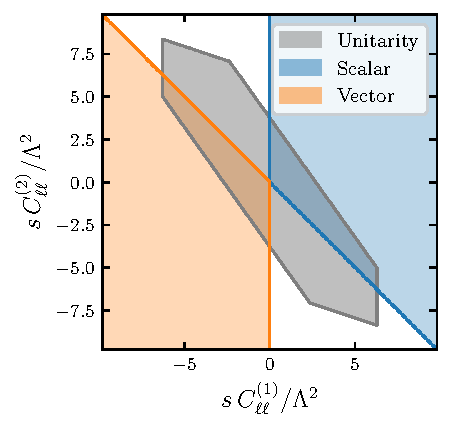
\includegraphics[scale = 0.75]{images/flavor/Oll_mfv.pdf}
    \caption{Partial-wave unitarity bounds and sum-rule constraints (under scalar and vector dominance) for the operator $O_{\ell\ell}$ under MFV, where $[C_{\ell\ell}]_{prst} = C_{\ell\ell}^{(1)}\delta_{pr}\delta_{st} + C_{\ell\ell}^{(2)}\delta_{pt}\delta_{rs}$.}
    \label{fig:Oll_mfv}
\end{figure}

\begin{figure}[p]
    \centering
    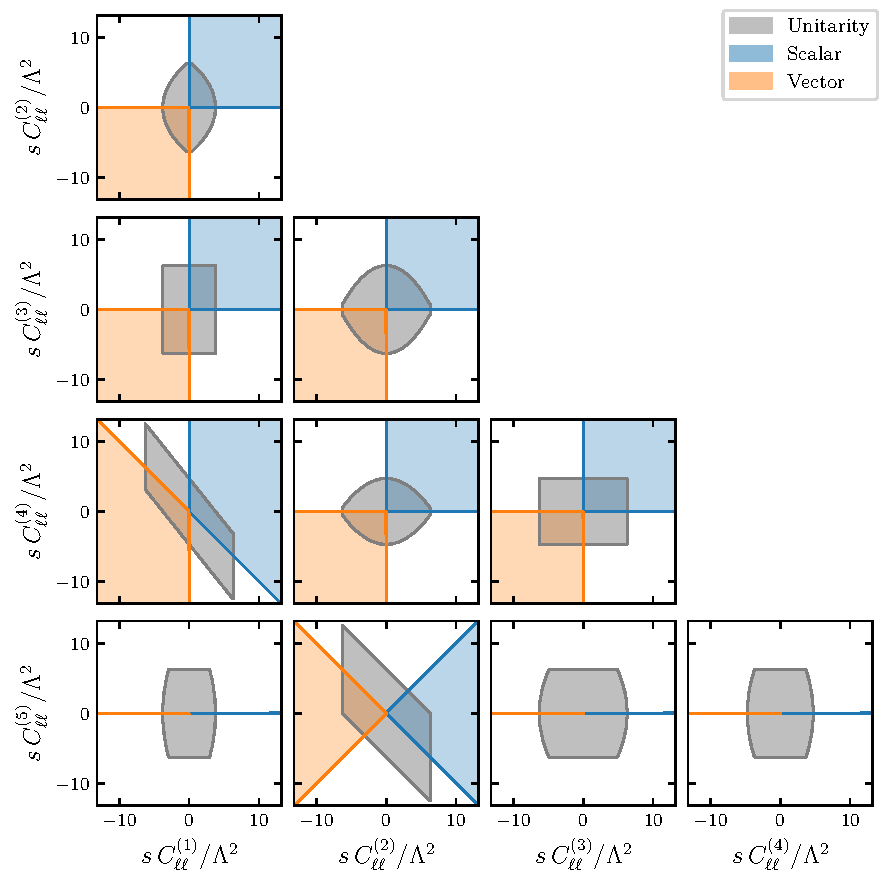
\includegraphics[scale = 0.75]{images/flavor/Oll_u2.pdf}
    \caption{Partial-wave unitarity bounds and sum-rule constraints (under scalar and vector dominance) for the operator $O_{\ell\ell}$ under $U(2)^5$ flavor symmetry, where $[C_{\ell\ell}]_{prst} =
            C_{\ell\ell}^{(1)}\Pij{p}{r}{a}\Pij{s}{t}{b}
            + C_{\ell\ell}^{(2)}(\Pij{s}{t}{a}\delta_{p3}\delta_{3r} + \Pij{p}{r}{a}\delta_{s3}\delta_{3t})
            + C_{\ell\ell}^{(3)}\delta_{p3}\delta_{3r}\delta_{s3}\delta_{3t}
            + C_{\ell\ell}^{(4)}\Pij{s}{r}{a}\Pij{p}{t}{b}
            + C_{\ell\ell}^{(5)}(\Pij{p}{t}{a}\delta_{s3}\delta_{3r} + \Pij{s}{r}{a}\delta_{p3}\delta_{3t})$. The regions shown are two-dimensional slices of the full allowed region, obtained by setting to zero all the independent coefficients other than the two displayed.}
    \label{fig:Oll_u2}
\end{figure}

\begin{figure}[p]
    \centering
    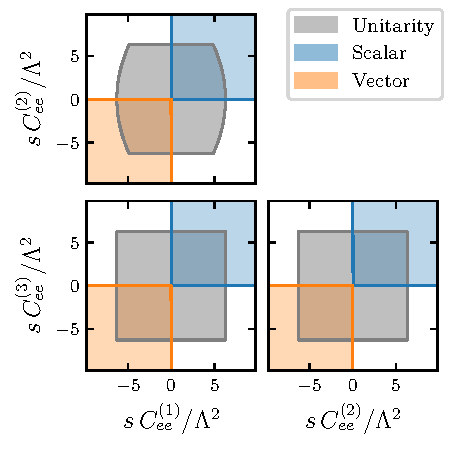
\includegraphics[scale = 0.75]{images/flavor/Oee_u2.pdf}
    \caption{Partial-wave unitarity bounds and sum-rule constraints (under scalar and vector dominance) for the operator $O_{ee}$ under $U(2)^5$ flavor symmetry, where $[C_{ee}]_{prst} =
            C_{ee}^{(1)}\Pij{p}{r}{a}\Pij{s}{t}{b}
            + C_{ee}^{(2)}(\Pij{s}{t}{a}\delta_{p3}\delta_{3r} + \Pij{p}{r}{a}\delta_{s3}\delta_{3t}) + C_{ee}^{(3)}\delta_{p3}\delta_{3r}\delta_{s3}\delta_{3t}$. The regions shown are two-dimensional slices of the full allowed region, obtained by setting to zero all the independent coefficients other than the two displayed.}
    \label{fig:Oee_u2}
\end{figure}

\begin{figure}[p]
    \centering
    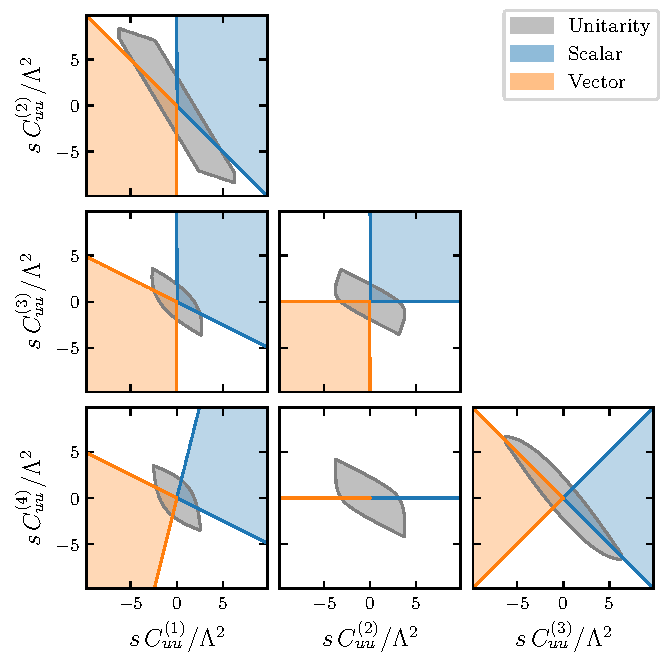
\includegraphics[scale = 0.75]{images/flavor/Ouu_mfv.pdf}
    \caption{Partial-wave unitarity bounds and sum-rule constraints (under scalar and vector dominance) for the operators $O_{uu}$ under MFV, where $[C_{uu}]_{prst} =
            C_{uu}^{(1)}\delta_{pr}\delta_{st}
            + C_{uu}^{(2)}\delta_{pt}\delta_{sr}
            + C_{uu}^{(3)}((Y_u^\dagger Y_u)_{st}\delta_{pr} + (Y_u^\dagger Y_u)_{pr}\delta_{st})+ C_{uu}^{(4)}((Y_u^\dagger Y_u)_{sr}\delta_{pt} + (Y_u^\dagger Y_u)_{pt}\delta_{sr})$. The regions shown are two-dimensional slices of the full allowed region, obtained by setting to zero all the independent coefficients other than the two displayed.}
    \label{fig:Ouu_mfv}
\end{figure}

\begin{figure}[p]
    \centering
    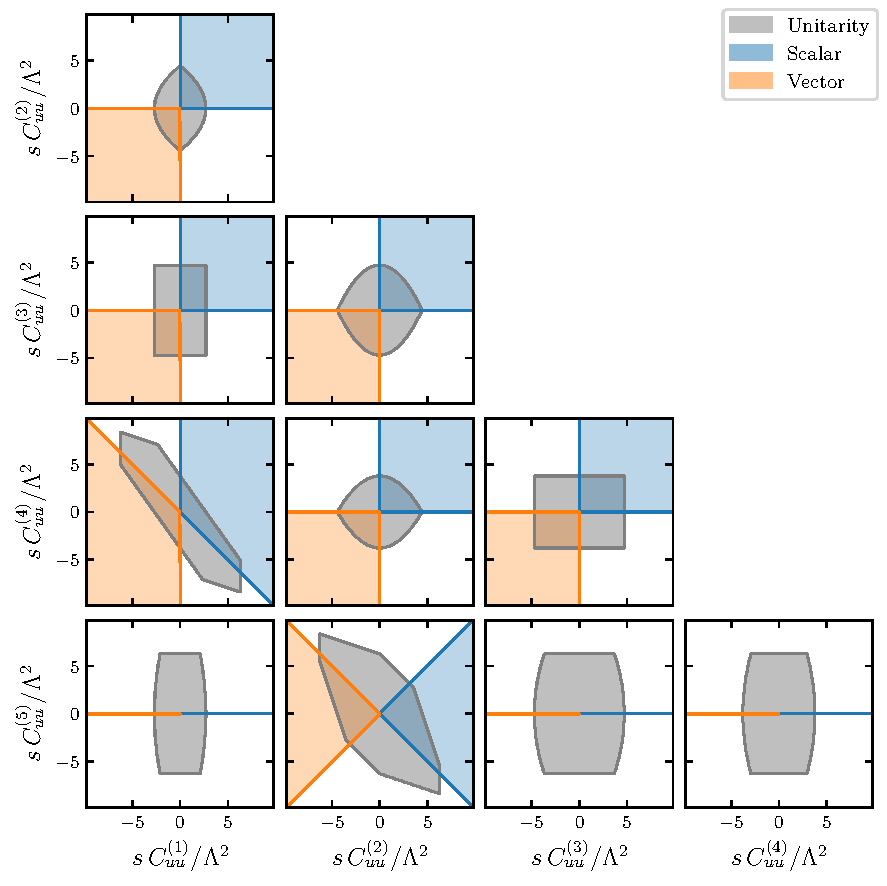
\includegraphics[scale = 0.75]{images/flavor/Ouu_u2.pdf}
    \caption{Partial-wave unitarity bounds and sum-rule constraints (under scalar and vector dominance) for the operators $O_{uu}$ under $U(2)^5$ flavor symmetry, where $[C_{uu}]_{prst} =
            C_{uu}^{(1)}\Pij{p}{r}{a}\Pij{s}{t}{b}
            + C_{uu}^{(2)}(\Pij{s}{t}{a}\delta_{p3}\delta_{3r} + \Pij{p}{r}{a}\delta_{s3}\delta_{3t})
            + C_{uu}^{(3)}\delta_{p3}\delta_{3r}\delta_{s3}\delta_{3t}
            + C_{uu}^{(4)}\Pij{p}{t}{a}\Pij{s}{r}{b}
            + C_{uu}^{(5)}(\Pij{s}{r}{a}\delta_{p3}\delta_{3t} + \Pij{p}{t}{a}\delta_{s3}\delta_{3r})$. Same decomposition and plots are valid also for $O_{dd}$. The regions shown are two-dimensional slices of the full allowed region, obtained by setting to zero all the independent coefficients other than the two displayed.}
    \label{fig:Ouu_u2}
\end{figure}

\begin{figure}[p]
    \centering
    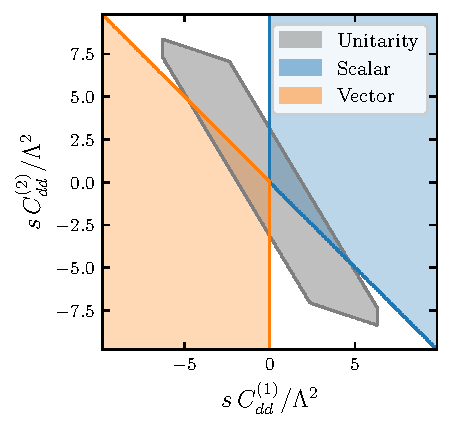
\includegraphics[scale = 0.75]{images/flavor/Odd_mfv.pdf}
    \caption{Partial-wave unitarity bounds and sum-rule constraints (under scalar and vector dominance) for the operators $O_{dd}$ under MFV, where $[C_{dd}]_{prst} =
            C_{dd}^{(1)}\delta_{pr}\delta_{st}
            + C_{dd}^{(2)}\delta_{pt}\delta_{sr}
            $.}
    \label{fig:Odd_mfv}
\end{figure}

\begin{figure}[p]
    \centering
    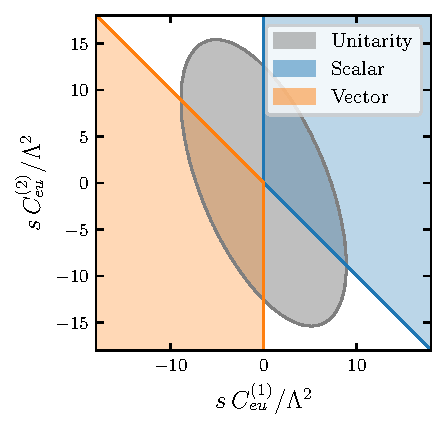
\includegraphics[scale = 0.75]{images/flavor/Oeu_mfv.pdf}
    \caption{Partial-wave unitarity bounds and sum-rule constraints (under scalar and vector dominance) for the operators $O_{eu}$ under MFV, where $[C_{eu}]_{prst} =
            C_{eu}^{(1)}\delta_{pr}\delta_{st}
            + C_{eu}^{(2)}\delta_{pr}(Y_u^\dagger Y_u)_{st}
            $.}
    \label{fig:Oeu_mfv}
\end{figure}

\begin{figure}[p]
    \centering
    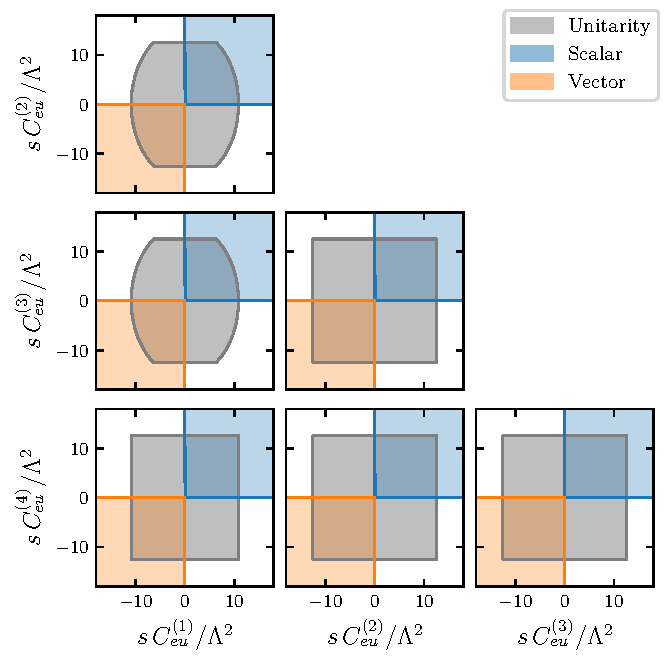
\includegraphics[scale = 0.75]{images/flavor/Oeu_u2.pdf}
    \caption{Partial-wave unitarity bounds and sum-rule constraints (under scalar and vector dominance) for the operators $O_{eu}$ under $U(2)^5$ flavor symmetry, where $[C_{eu}]_{prst} =
            C_{eu}^{(1)}\Pij{p}{r}{a}\Pij{s}{t}{b}
            + C_{eu}^{(2)}\delta_{p3}\delta_{3r}\Pij{s}{t}{a} + C_{eu}^{(3)}\delta_{s3}\delta_{3t}\Pij{p}{r}{a}
            + C_{eu}^{(4)}\delta_{p3}\delta_{3r}\delta_{s3}\delta_{3t}$. Same decomposition and plots are valid also for $O_{ed}$. The regions shown are two-dimensional slices of the full allowed region, obtained by setting to zero all the independent coefficients other than the two displayed.}
    \label{fig:Oeu_u2}
\end{figure}

\begin{figure}[p]
    \centering
    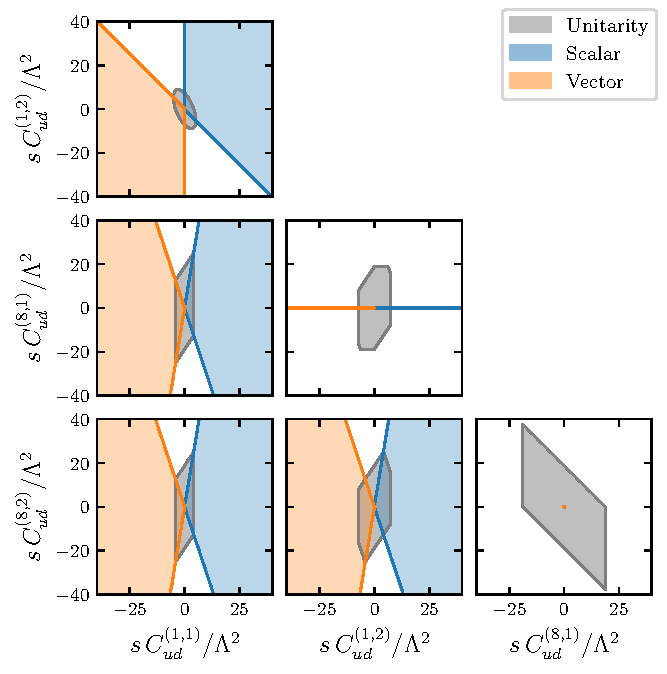
\includegraphics[scale = 0.75]{images/flavor/Oud_mfv.pdf}
    \caption{Partial-wave unitarity bounds and sum-rule constraints (under scalar and vector dominance) for the operators $O_{ud}^{(1,8)}$ under MFV, where $[C_{ud}^{(i)}]_{prst} =
            C_{ud}^{(i,1)}\delta_{pr}\delta_{st}
            + C_{ud}^{(i,2)}(Y_u^\dagger Y_u)_{pr}\delta_{st}$, $i=1,8$. The regions shown are two-dimensional slices of the full allowed region, obtained by setting to zero all the independent coefficients other than the two displayed.}
    \label{fig:Oud_mfv}
\end{figure}

\begin{figure}[p]
    \centering
    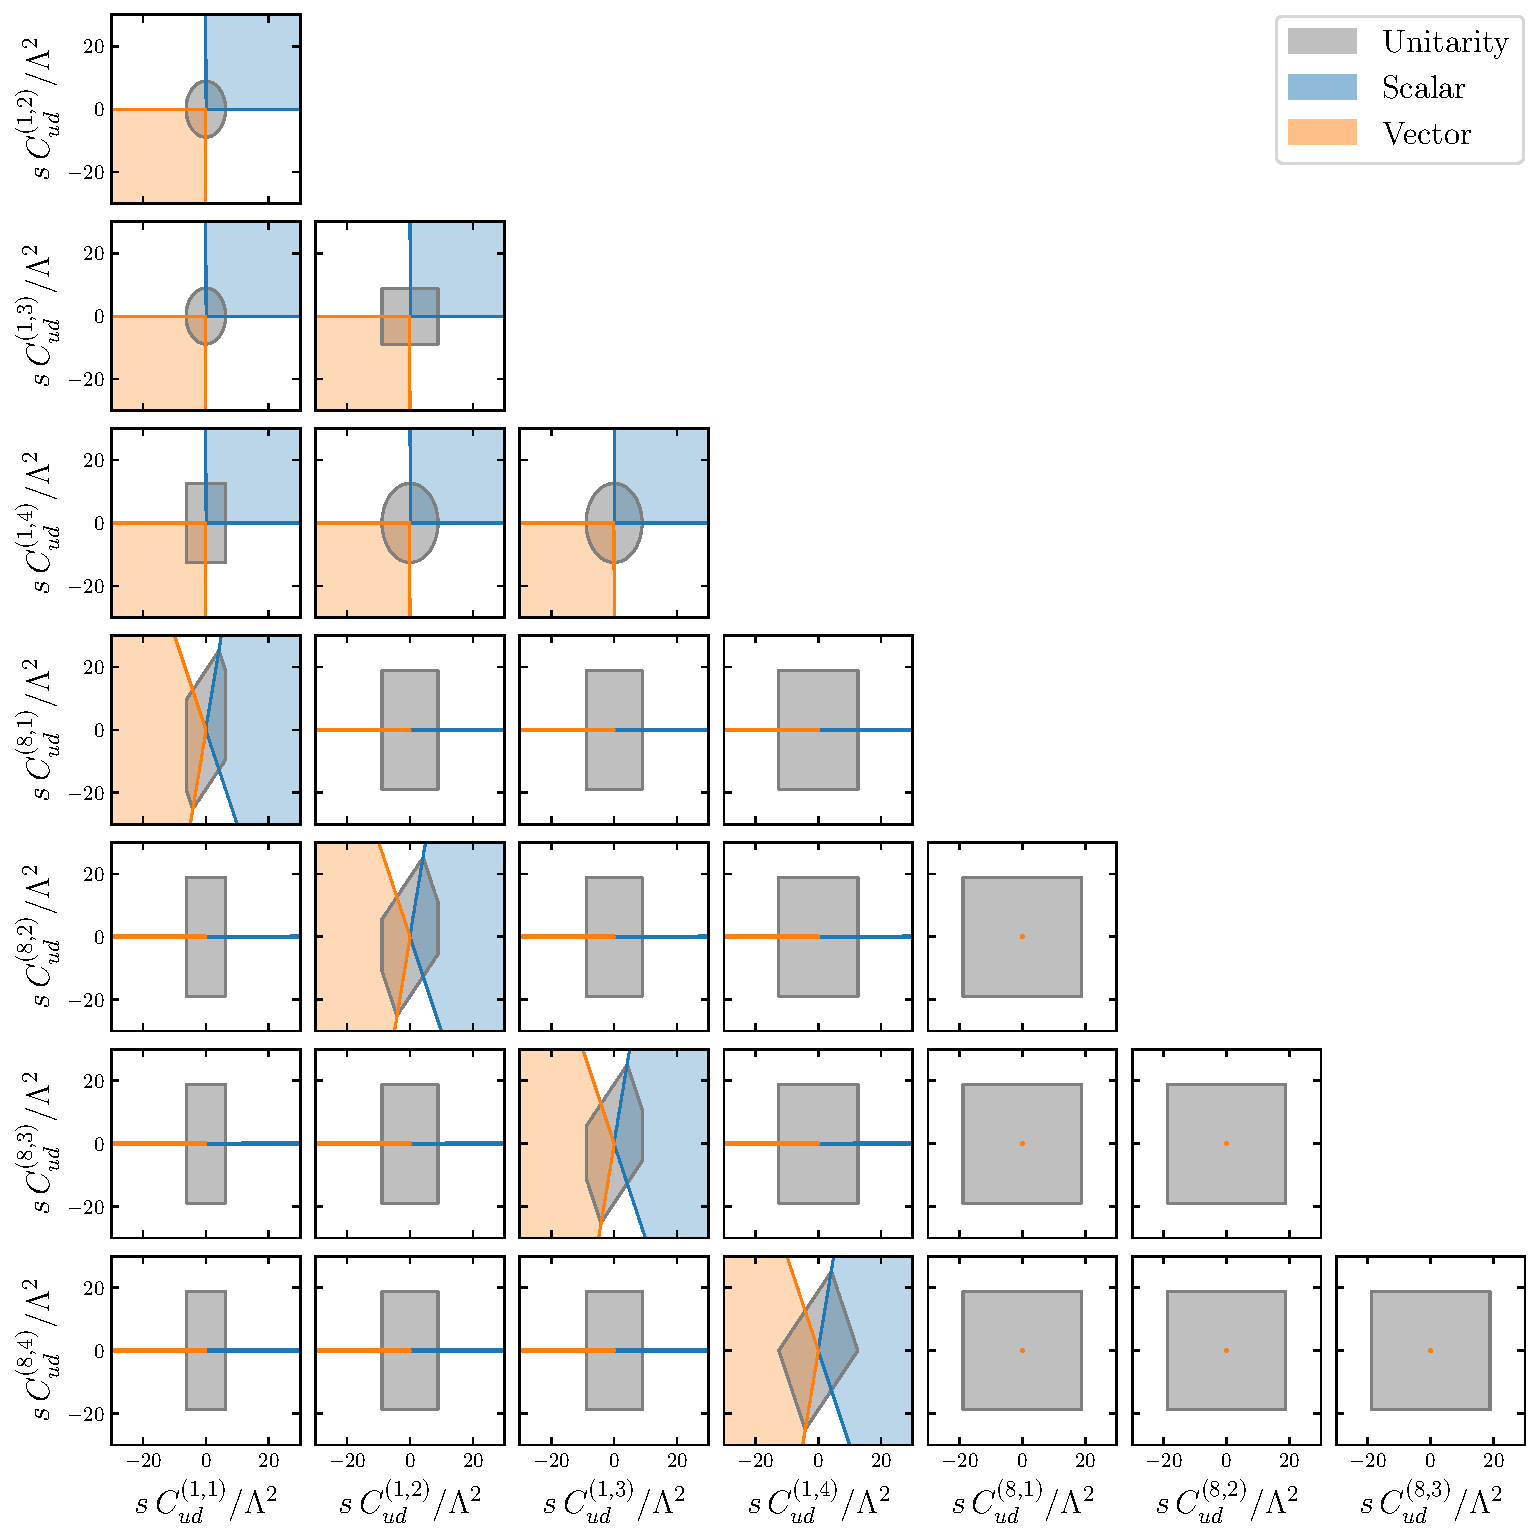
\includegraphics[width=\linewidth]{images/flavor/Oud_u2.pdf}
    \caption{Partial-wave unitarity bounds and sum-rule constraints (under scalar and vector dominance) for the operators $O_{ud}^{(1,8)}$ under $U(2)^5$ flavor symmetry, where $[C_{ud}^{(i)}]_{prst} =
            C_{ud}^{(i,1)}\Pij{p}{r}{a}\Pij{s}{t}{b}
            + C_{ud}^{(i,2)}\Pij{s}{t}{a}\delta_{p3}\delta_{3r}+ C_{ud}^{(i,3)}\Pij{p}{r}{a}\delta_{s3}\delta_{3t}
            + C_{ud}^{(i,4)}\delta_{p3}\delta_{3r}\delta_{s3}\delta_{3t}$, $i=1,8$. The regions shown are two-dimensional slices of the full allowed region, obtained by setting to zero all the independent coefficients other than the two displayed.}
    \label{fig:Oud_u2}
\end{figure}

\begin{figure}[p]
    \centering
    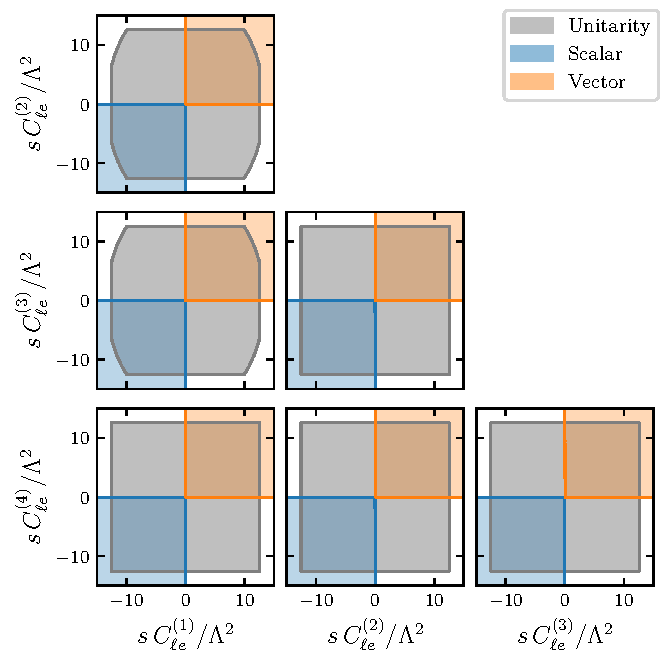
\includegraphics[scale = 0.75]{images/flavor/Ole_u2.pdf}
    \caption{Partial-wave unitarity bounds and sum-rule constraints (under scalar and vector dominance) for the operators $O_{\ell e}$ under $U(2)^5$ flavor symmetry, where $[C_{\ell e}]_{prst} =
            C_{\ell e}^{(1)}\Pij{p}{r}{a}\Pij{s}{t}{a}
            + C_{\ell e}^{(2)}\Pij{s}{t}{a}\delta_{p3}\delta_{3r}+ C_{\ell e}^{(3)}\Pij{p}{r}{a}\delta_{s3}\delta_{3t}
            + C_{\ell e}^{(4)}\delta_{p3}\delta_{3r}\delta_{s3}\delta_{3t}$. The regions shown are two-dimensional slices of the full allowed region, obtained by setting to zero all the independent coefficients other than the two displayed.}
    \label{fig:Ole_u2}
\end{figure}

\begin{figure}[p]
    \centering
    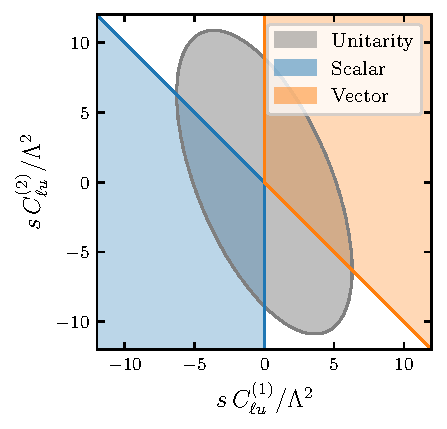
\includegraphics[scale = 0.75]{images/flavor/Olu_mfv.pdf}
    \caption{Partial-wave unitarity bounds and sum-rule constraints (under scalar and vector dominance) for the operators $O_{\ell u}$ under MFV, where $[C_{\ell u}]_{prst} = C_{\ell u}^{(1)}\delta_{pr}\delta_{st} + C_{\ell u}^{(2)}\delta_{pr}(Y_u^\dagger Y_u)_{st}$.}
    \label{fig:Olu_mfv}
\end{figure}

\begin{figure}[p]
    \centering
    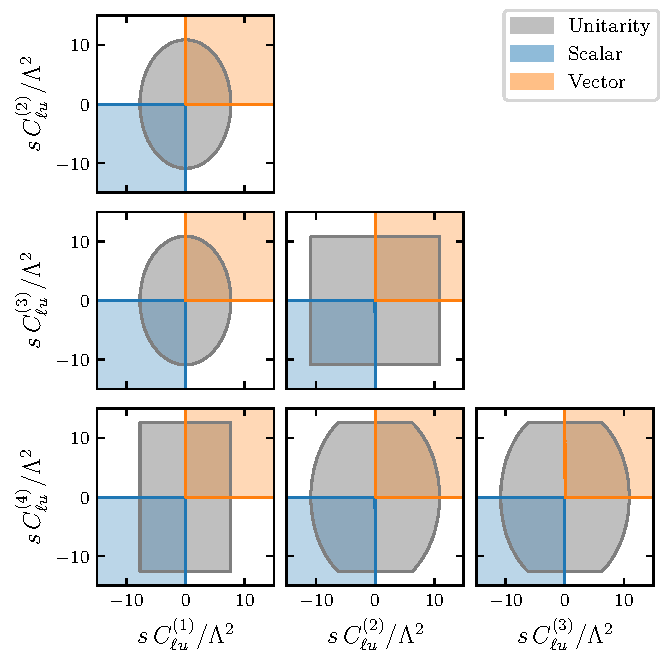
\includegraphics[scale = 0.75]{images/flavor/Olu_u2.pdf}
    \caption{Partial-wave unitarity bounds and sum-rule constraints (under scalar and vector dominance) for the operators $O_{\ell u}$ under $U(2)^5$ flavor symmetry, where $[C_{\ell u}]_{prst} =
            C_{\ell u}^{(1)}\Pij{p}{r}{a}\Pij{s}{t}{a}
            + C_{\ell u}^{(2)}\Pij{s}{t}{a}\delta_{p3}\delta_{3r}+ C_{\ell u}^{(3)}\Pij{p}{r}{a}\delta_{s3}\delta_{3t}
            + C_{\ell u}^{(4)}\delta_{p3}\delta_{3r}\delta_{s3}\delta_{3t}$. Same decomposition and plots are valid also for $O_{\ell d}$. The regions shown are two-dimensional slices of the full allowed region, obtained by setting to zero all the independent coefficients other than the two displayed.}
    \label{fig:Olu_u2}
\end{figure}

\begin{figure}[p]
    \centering
    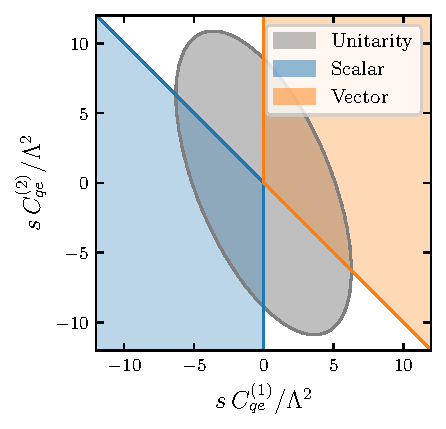
\includegraphics[scale = 0.75]{images/flavor/Oqe_mfv.pdf}
    \caption{Partial-wave unitarity bounds and sum-rule constraints (under scalar and vector dominance) for the operators $O_{qe}$ under MFV, where $[C_{qe}]_{prst} = C_{qe}^{(1)}\delta_{pr}\delta_{st} + C_{qe}^{(2)}(Y_u Y_u^\dagger)_{pr}\delta_{st}$.}
    \label{fig:Oqe_mfv}
\end{figure}

\begin{figure}[p]
    \centering
    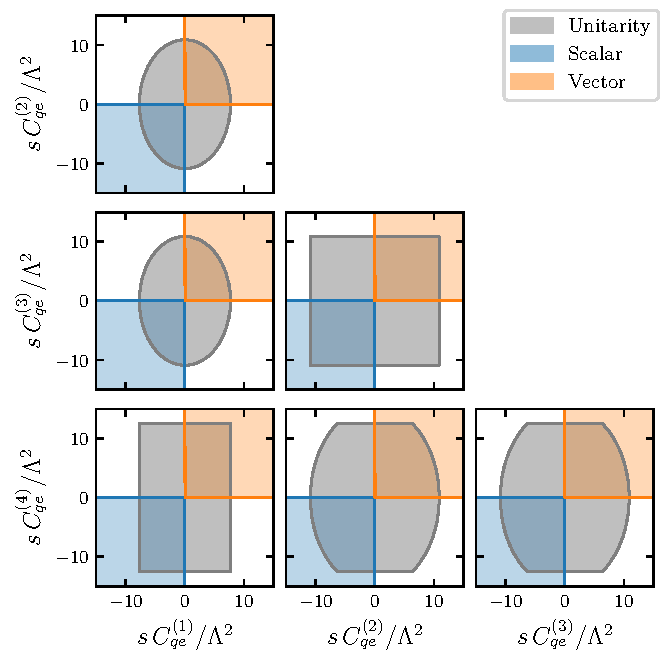
\includegraphics[scale = 0.75]{images/flavor/Oqe_u2.pdf}
    \caption{Partial-wave unitarity bounds and sum-rule constraints (under scalar and vector dominance) for the operators $O_{qe}$ under $U(2)^5$ flavor symmetry, where $[C_{qe}]_{prst} =
            C_{qe}^{(1)}\Pij{p}{r}{a}\Pij{s}{t}{a}
            + C_{qe}^{(2)}\Pij{s}{t}{a}\delta_{p3}\delta_{3r}+ C_{qe}^{(3)}\Pij{p}{r}{a}\delta_{s3}\delta_{3t}
            + C_{qe}^{(4)}\delta_{p3}\delta_{3r}\delta_{s3}\delta_{3t}$. The regions shown are two-dimensional slices of the full allowed region, obtained by setting to zero all the independent coefficients other than the two displayed.}
    \label{fig:Oqe_u2}
\end{figure}

\begin{figure}[p]
    \centering
    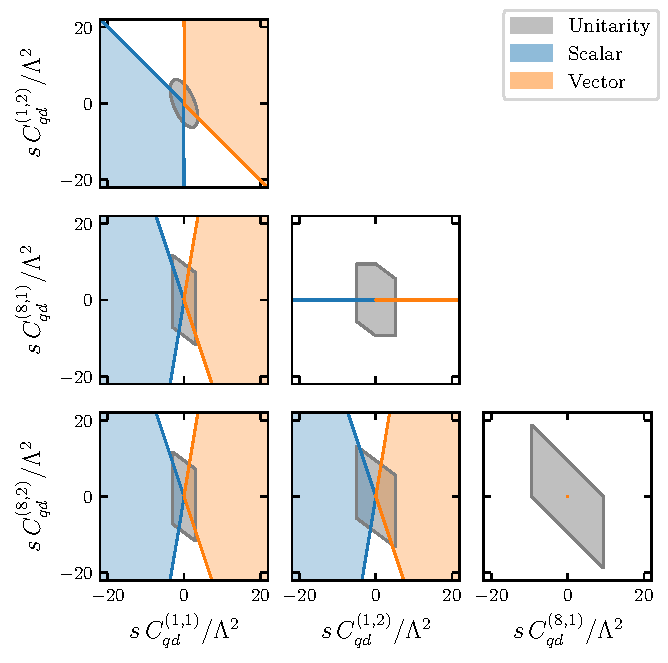
\includegraphics[scale = 0.75]{images/flavor/Oqd_mfv.pdf}
    \caption{Partial-wave unitarity bounds and sum-rule constraints (under scalar and vector dominance) for the operators $O_{qd}^{(1,8)}$ under MFV, where $[C_{qd}^{(i)}]_{prst} =
            C_{qd}^{(i,1)}\delta_{pr}\delta_{st}
            + C_{qd}^{(i,2)}(Y_u Y_u^\dagger)_{pr}\delta_{st}$, $i=1,8$. The regions shown are two-dimensional slices of the full allowed region, obtained by setting to zero all the independent coefficients other than the two displayed.}
    \label{fig:Oqd_mfv}
\end{figure}

\begin{figure}[p]
    \centering
    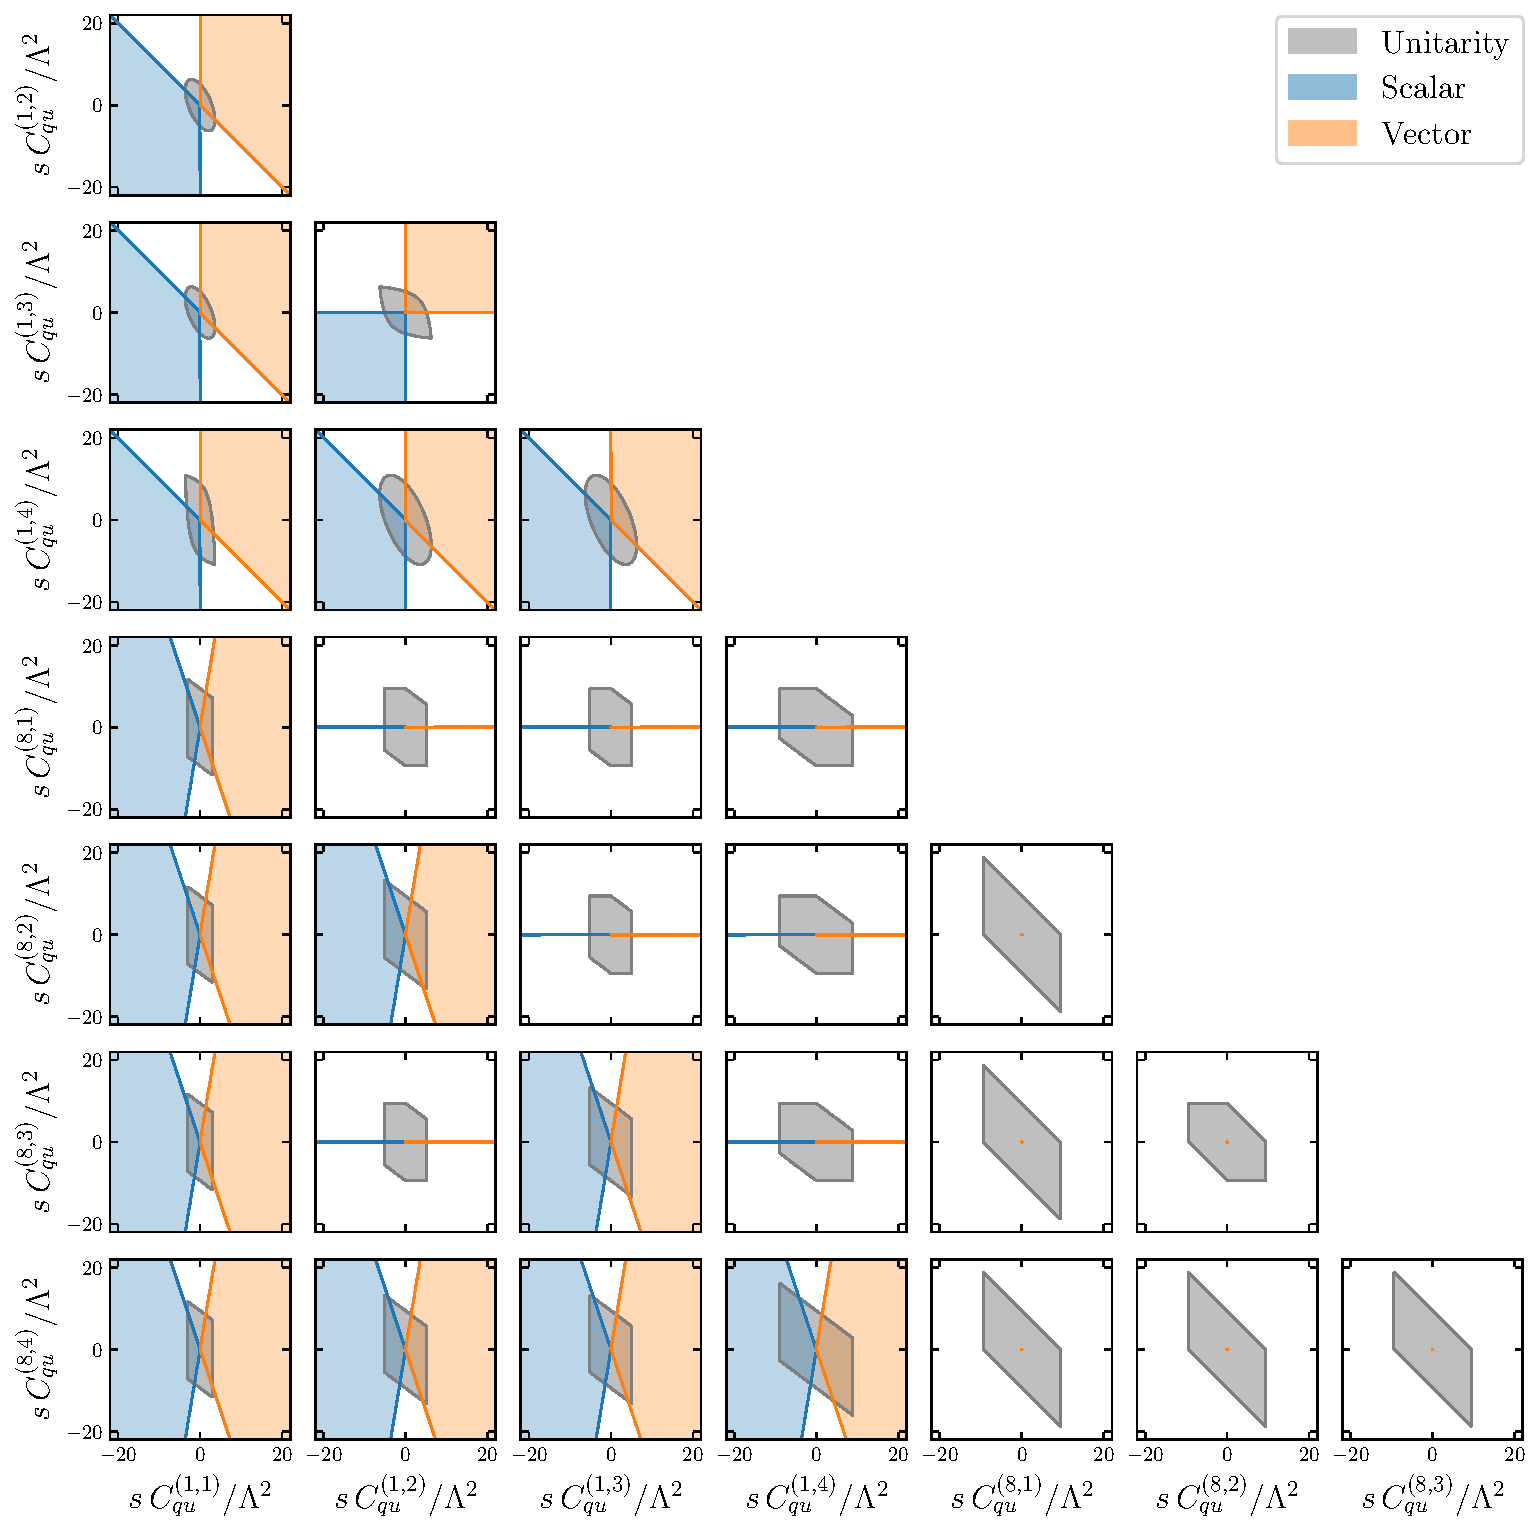
\includegraphics[width=\linewidth]{images/flavor/Oqu_mfv.pdf}
    \caption{Partial-wave unitarity bounds and sum-rule constraints (under scalar and vector dominance) for the operators $O_{qu}^{(1,8)}$ under MFV, where $[C_{qu}^{(i)}]_{prst} =
            C_{qu}^{(i,1)}\delta_{pr}\delta_{st}
            + C_{qu}^{(i,2)}(Y_u Y_u^\dagger)_{pr}\delta_{st}+ C_{qu}^{(i,3)}\delta_{pr}(Y_u^\dagger Y_u)_{st}
            + C_{qu}^{(i,4)}(Y_u)_{pt}(Y_u^\dagger)_{sr}$, $i=1,8$. The regions shown are two-dimensional slices of the full allowed region, obtained by setting to zero all the independent coefficients other than the two displayed.}
    \label{fig:Oqu_mfv}
\end{figure}

\begin{figure}[p]
    \centering
    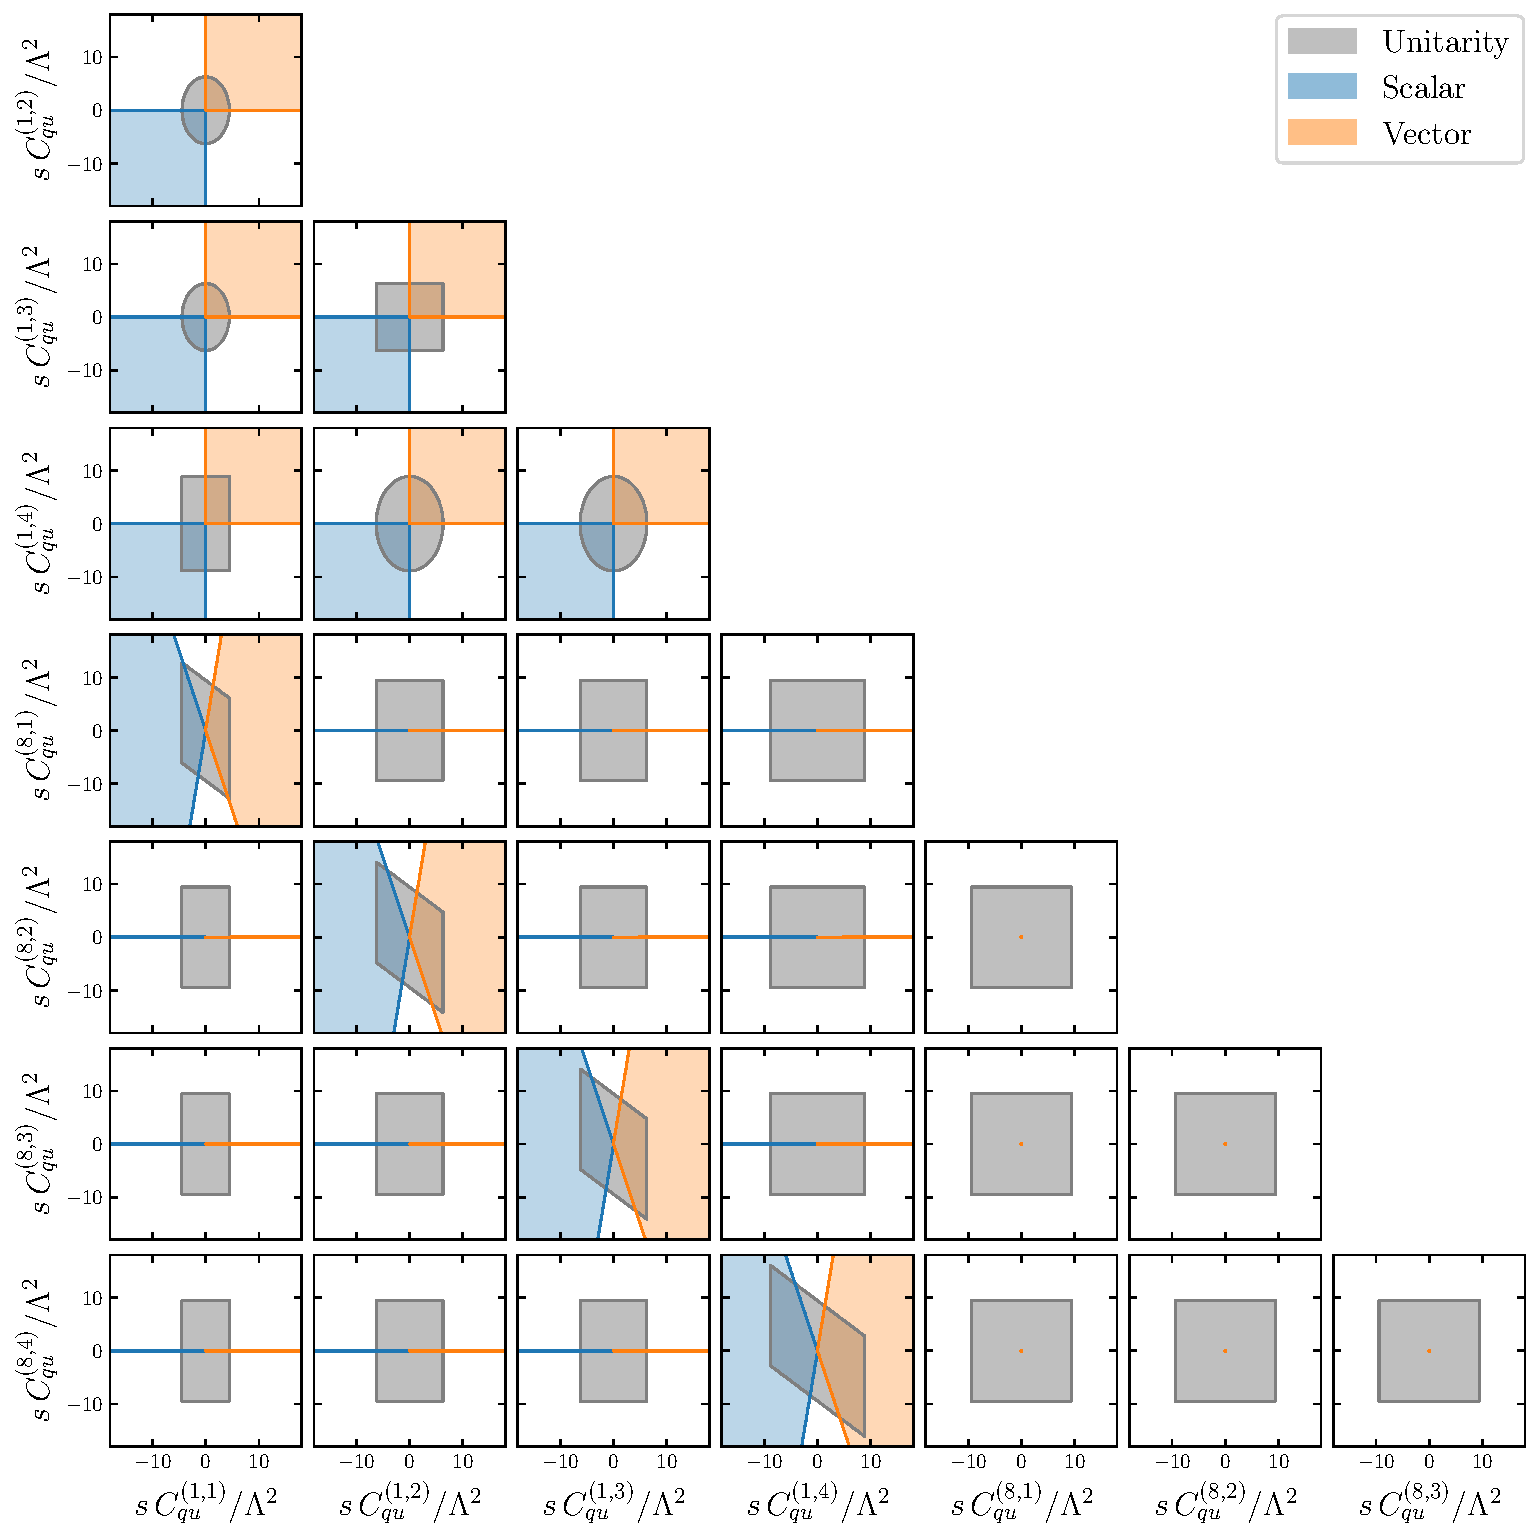
\includegraphics[width=\linewidth]{images/flavor/Oqu_u2.pdf}
    \caption{Partial-wave unitarity bounds and sum-rule constraints (under scalar and vector dominance) for the operators $O_{qu}^{(1,8)}$ under $U(2)^5$ flavor symmetry, where $[C_{qu}^{(i)}]_{prst} =
            C_{qu}^{(i,1)}\Pij{p}{r}{a}\Pij{s}{t}{a}
            + C_{qu}^{(i,2)}\Pij{s}{t}{a}\delta_{p3}\delta_{3r}+ C_{qu}^{(i,3)}\Pij{p}{r}{a}\delta_{s3}\delta_{3t}
            + C_{qu}^{(i,4)}\delta_{p3}\delta_{3r}\delta_{s3}\delta_{3t}$, $i=1,8$. Same decomposition and plots are valid also for $O_{qd}^{(1,8)}$. The regions shown are two-dimensional slices of the full allowed region, obtained by setting to zero all the independent coefficients other than the two displayed.}
    \label{fig:Oqu_u2}
\end{figure}


\end{subappendices}